\RequirePackage{currfile}
\documentclass[12pt]{beamer}
\usepackage[utf8]{inputenc}
\usepackage[spanish]{babel}
\usepackage{standalone}
\usepackage{color}
\usepackage{siunitx}
\usepackage{hyperref}
%\hypersetup{colorlinks,linkcolor=,urlcolor=blue}
%\hypersetup{colorlinks,urlcolor=blue}
\usepackage{xcolor,soul}
\usepackage{etoolbox}
\usepackage{amsmath}
\usepackage{amsthm}
\usepackage{physics}
\usepackage{multicol}
\usepackage{bookmark}
\usepackage{longtable}
\usepackage{listings}
\usepackage{graphicx}
\usepackage{tikz}
\usepackage[siunitx, RPvoltages]{circuitikz}
\usetikzlibrary{arrows, patterns, matrix, backgrounds, decorations, shapes, decorations.markings, decorations.pathmorphing}
\usepackage[autostyle,spanish=mexican]{csquotes}
\usepackage[os=win]{menukeys}
\usepackage{pifont}
\usepackage{pbox}
\usepackage{caption}
\captionsetup{font=scriptsize,labelfont=scriptsize}
%\usepackage[sfdefault]{roboto}  %% Option 'sfdefault' only if the base font of the document is to be sans serif

%Sección de definición de colores
\definecolor{ao}{rgb}{0.0, 0.5, 0.0}
\definecolor{bisque}{rgb}{1.0, 0.89, 0.77}
\definecolor{amber}{rgb}{1.0, 0.75, 0.0}
\definecolor{armygreen}{rgb}{0.29, 0.33, 0.13}
\definecolor{alizarin}{rgb}{0.82, 0.1, 0.26}
\definecolor{cadetblue}{rgb}{0.37, 0.62, 0.63}
\definecolor{deepblue}{rgb}{0,0,0.5}
\definecolor{brown}{rgb}{0.59, 0.29, 0.0}
\definecolor{OliveGreen}{rgb}{0,0.25,0}


\usefonttheme[onlymath]{serif}
%Sección de definición de nuevos comandos

\newcommand*{\TitleParbox}[1]{\parbox[c]{1.75cm}{\raggedright #1}}%
\newcommand{\python}{\texttt{python}}
\newcommand{\textoazul}[1]{\textcolor{blue}{#1}}
\newcommand{\azulfuerte}[1]{\textcolor{blue}{\textbf{#1}}}
\newcommand{\funcionazul}[1]{\textcolor{blue}{\textbf{\texttt{#1}}}}
\newcommand{\ptilde}[1]{\ensuremath{{#1}^{\prime}}}
\newcommand{\ptildosargs}[2]{\ensuremath{{#1}^{\prime \, ({#2})}}}
\newcommand{\stilde}[1]{\ensuremath{{#1}^{\prime \prime}}}
\newcommand{\ttilde}[1]{\ensuremath{{#1}^{\prime \prime \prime}}}
\newcommand{\ntilde}[2]{\ensuremath{{#1}^{(#2)}}}
\renewcommand{\arraystretch}{1.5}

\newcounter{saveenumi}
\newcommand{\seti}{\setcounter{saveenumi}{\value{enumi}}}
\newcommand{\conti}{\setcounter{enumi}{\value{saveenumi}}}
\renewcommand{\rmdefault}{cmr}% cmr = Computer Modern Roman

\linespread{1.5}

\usefonttheme{professionalfonts}
%\usefonttheme{serif}
\DeclareGraphicsExtensions{.pdf,.png,.jpg}


%Sección para el tema de beamer, con el theme, usercolortheme y sección de footers
\mode<presentation>
{
  \usetheme{Warsaw}
  \setbeamertemplate{headline}{}
  %\useoutertheme{infolines}
  \useoutertheme{default}
  \usecolortheme{seahorse}
  \setbeamercovered{invisible}
  % or whatever (possibly just delete it)
  \setbeamertemplate{section in toc}[sections numbered]
  \setbeamertemplate{subsection in toc}[subsections numbered]
  \setbeamertemplate{subsection in toc}{\leavevmode\leftskip=3.2em\rlap{\hskip-2em\inserttocsectionnumber.\inserttocsubsectionnumber}\inserttocsubsection\par}
  \setbeamercolor{section in toc}{fg=blue}
  \setbeamercolor{subsection in toc}{fg=blue}
  \setbeamercolor{frametitle}{fg=blue}

  \setbeamertemplate{footline}
  %\beamertemplatenavigationsymbolsempty
}

\makeatletter
\setbeamercolor{section in foot}{bg=gray!30, fg=black!90!orange}
\setbeamercolor{subsection in foot}{bg=blue!30!yellow, fg=red}
\setbeamertemplate{footline}
{
  \leavevmode%
  \hbox{%
  \begin{beamercolorbox}[wd=.333333\paperwidth,ht=2.25ex,dp=1ex,center]{section in foot}%
    \usebeamerfont{section in foot} \insertsection
  \end{beamercolorbox}}%
  \begin{beamercolorbox}[wd=.333333\paperwidth,ht=2.25ex,dp=1ex,center]{subsection in foot}%
    \usebeamerfont{subsection in foot}  \insertsubsection
  \end{beamercolorbox}%
  \begin{beamercolorbox}[wd=.333333\paperwidth,ht=2.25ex,dp=1ex,right]{date in head/foot}%
    \usebeamerfont{date in head/foot} \insertshortdate{} \hspace*{2em}
    \insertframenumber{} / \inserttotalframenumber \hspace*{2ex} 
  \end{beamercolorbox}}%
  \vskip0pt%
\makeatother  

\makeatletter
\patchcmd{\beamer@sectionintoc}
  {\vfill}
  {\vskip\itemsep}
  {}
  {}
\makeatother

% \makeatletter
% \patchcmd{\hyper@link@}
%   {{\Hy@tempb}{#4}}
%   {{\Hy@tempb}{\ul{#4}}}
%   {}{}
% \makeatother


% Sección para el código

\definecolor{Code}{rgb}{0,0,0}
\definecolor{Keywords}{rgb}{255,0,0}
\definecolor{Strings}{rgb}{255,0,255}
\definecolor{Comments}{rgb}{0,0,255}
\definecolor{Numbers}{rgb}{255,128,0}

\DeclareCaptionFont{white}{\color{white}}
\DeclareCaptionFormat{listing}{\colorbox{gray}{\parbox{0.99\textwidth}{#1#2#3}}}
\captionsetup[lstlisting]{format=listing,labelfont=white,textfont=white}
\renewcommand{\lstlistingname}{Código}

\lstset{
basicstyle=\ttfamily,
columns=fullflexible,
breaklines=true
}

\lstdefinestyle{codigopython}{%
  language=Python,                % choose the language of the code
  %basicstyle=\footnotesize\small,       % the size of the fonts that are used for the code
  numbers=left,                   % where to put the line-numbers
  numberstyle=\scriptsize,      % the size of the fonts that are used for the line-numbers
  stepnumber=1,                   % the step between two line-numbers. If it is 1 each line will be numbered
  numbersep=5pt,                  % how far the line-numbers are from the code
  backgroundcolor=\color{white},  % choose the background color. You must add \usepackage{color}
  showspaces=false,               % show spaces adding particular underscores
  showstringspaces=false,         % underline spaces within strings
  showtabs=false,                 % show tabs within strings adding particular underscores
  frame=single,   		% adds a frame around the code
  tabsize=2,  		% sets default tabsize to 2 spaces
  captionpos=t,   		% sets the caption-position to bottom
  breaklines=true,    	% sets automatic line breaking
  breakatwhitespace=false,    % sets if automatic breaks should only happen at whitespace
  escapeinside={\#},  % if you want to add a comment within your code
  stringstyle =\color{OliveGreen},
  texcl = true,
  %otherkeywords={{as}},             % Add keywords here
  keywordstyle = \color{blue},
  commentstyle = \color{black},
  identifierstyle = \color{black},
  % literate=%
  %         {á}{{\'a}}1
  %         {é}{{\'e}}1
  %         {í}{{\'i}}1
  %         {ó}{{\'o}}1
  %         {ú}{{\'u}}1
  %
  %keywordstyle=\ttb\color{deepblue}
  %fancyvrb = true,
literate={0}{{\textcolor{red}{0}}}{1}%
            {1}{{\textcolor{red}{1}}}{1}%
            {2}{{\textcolor{red}{2}}}{1}%
            {3}{{\textcolor{red}{3}}}{1}%
            {4}{{\textcolor{red}{4}}}{1}%
            {5}{{\textcolor{red}{5}}}{1}%
            {6}{{\textcolor{red}{6}}}{1}%
            {7}{{\textcolor{red}{7}}}{1}%
            {8}{{\textcolor{red}{8}}}{1}%
            {9}{{\textcolor{red}{9}}}{1}%
            {.0}{{\textcolor{red}{.0}}}{2}% Following is to ensure that only periods
            {.1}{{\textcolor{red}{.1}}}{2}% followed by a digit are changed.
            {.2}{{\textcolor{red}{.2}}}{2}%
            {.3}{{\textcolor{red}{.3}}}{2}%
            {.4}{{\textcolor{red}{.4}}}{2}%
            {.5}{{\textcolor{red}{.5}}}{2}%
            {.6}{{\textcolor{red}{.6}}}{2}%
            {.7}{{\textcolor{red}{.7}}}{2}%
            {.8}{{\textcolor{red}{.8}}}{2}%
            {.9}{{\textcolor{red}{.9}}}{2}%
            {\ }{{ }}{1}% handle the space
        ,%
        %mathescape=true
        %escapeinside={*@}
        escapeinside={A_}{_B}
}

% \usepackage{courier}
\usepackage{listingsutf8}
\usepackage{listings}
\usepackage{xcolor}
\usepackage{textcomp}
\usepackage{color}
\definecolor{deepblue}{rgb}{0,0,0.5}
\definecolor{brown}{rgb}{0.59, 0.29, 0.0}
\definecolor{OliveGreen}{rgb}{0,0.25,0}
% \usepackage{minted}

\DeclareCaptionFont{white}{\color{white}}
\DeclareCaptionFormat{listing}{\colorbox{gray}{\parbox{0.98\textwidth}{#1#2#3}}}
\captionsetup[lstlisting]{format=listing,labelfont=white,textfont=white}
\renewcommand{\lstlistingname}{Código}


\definecolor{Code}{rgb}{0,0,0}
\definecolor{Keywords}{rgb}{255,0,0}
\definecolor{Strings}{rgb}{255,0,255}
\definecolor{Comments}{rgb}{0,0,255}
\definecolor{Numbers}{rgb}{255,128,0}

\makeatletter

\newif\iffirstchar\firstchartrue
\newif\ifstartedbyadigit
\newif\ifprecededbyequalsign

\newcommand\processletter
{%
  \ifnum\lst@mode=\lst@Pmode%
    \iffirstchar%
        \global\startedbyadigitfalse%
      \fi
      \global\firstcharfalse%
    \fi
}

\newcommand\processdigit
{%
  \ifnum\lst@mode=\lst@Pmode%
      \iffirstchar%
        \global\startedbyadigittrue%
      \fi
      \global\firstcharfalse%
  \fi
}

\lst@AddToHook{OutputOther}%
{%
  \lst@IfLastOtherOneOf{=}
    {\global\precededbyequalsigntrue}
    {}%
}

\lst@AddToHook{Output}%
{%
  \ifprecededbyequalsign%
      \ifstartedbyadigit%
        \def\lst@thestyle{\color{orange}}%
      \fi
    \fi
  \global\firstchartrue%
  \global\startedbyadigitfalse%
  \global\precededbyequalsignfalse%
}

\lstset{ 
language=Python,                % choose the language of the code
basicstyle=\footnotesize\ttfamily,       % the size of the fonts that are used for the code
numbers=left,                   % where to put the line-numbers
numberstyle=\scriptsize,      % the size of the fonts that are used for the line-numbers
stepnumber=1,                   % the step between two line-numbers. If it is 1 each line will be numbered
numbersep=5pt,                  % how far the line-numbers are from the code
backgroundcolor=\color{white},  % choose the background color. You must add \usepackage{color}
showspaces=false,               % show spaces adding particular underscores
showstringspaces=false,         % underline spaces within strings
showtabs=false,                 % show tabs within strings adding particular underscores
frame=single,   		% adds a frame around the code
tabsize=2,  		% sets default tabsize to 2 spaces
captionpos=t,   		% sets the caption-position to bottom
breaklines=true,    	% sets automatic line breaking
breakatwhitespace=false,    % sets if automatic breaks should only happen at whitespace
escapeinside={\#},  % if you want to add a comment within your code
stringstyle =\color{OliveGreen},
%otherkeywords={{as}},             % Add keywords here
keywordstyle = \color{blue},
commentstyle = \color{black},
identifierstyle = \color{black},
literate=%
         {á}{{\'a}}1
         {é}{{\'e}}1
         {í}{{\'i}}1
         {ó}{{\'o}}1
         {ú}{{\'u}}1
%
%keywordstyle=\ttb\color{deepblue}
%fancyvrb = true,
}

\lstdefinestyle{FormattedNumber}{%
    literate={0}{{\textcolor{red}{0}}}{1}%
             {1}{{\textcolor{red}{1}}}{1}%
             {2}{{\textcolor{red}{2}}}{1}%
             {3}{{\textcolor{red}{3}}}{1}%
             {4}{{\textcolor{red}{4}}}{1}%
             {5}{{\textcolor{red}{5}}}{1}%
             {6}{{\textcolor{red}{6}}}{1}%
             {7}{{\textcolor{red}{7}}}{1}%
             {8}{{\textcolor{red}{8}}}{1}%
             {9}{{\textcolor{red}{9}}}{1}%
             {.0}{{\textcolor{red}{.0}}}{2}% Following is to ensure that only periods
             {.1}{{\textcolor{red}{.1}}}{2}% followed by a digit are changed.
             {.2}{{\textcolor{red}{.2}}}{2}%
             {.3}{{\textcolor{red}{.3}}}{2}%
             {.4}{{\textcolor{red}{.4}}}{2}%
             {.5}{{\textcolor{red}{.5}}}{2}%
             {.6}{{\textcolor{red}{.6}}}{2}%
             {.7}{{\textcolor{red}{.7}}}{2}%
             {.8}{{\textcolor{red}{.8}}}{2}%
             {.9}{{\textcolor{red}{.9}}}{2}%
             {\ }{{ }}{1}% handle the space
         ,%
          %mathescape=true
          escapeinside={__}
          }



% %Se usa la plantilla Warsaw modificada con spruce
\mode<presentation>
{
  \usetheme{Warsaw}
  \setbeamertemplate{headline}{}
  \useoutertheme{default}
  \usecolortheme{seahorse}
  \setbeamercovered{invisible}
}
% \AtBeginSection[]
% {
% \begin{frame}<beamer>{Contenido}
% \normalfont\mdseries
% \tableofcontents[currentsection]
% \end{frame}
%}
% \makeatletter
\setbeamertemplate{footline}
%\setbeamercolor{title in head/foot}{fg=Green}
{
  \leavevmode%
  \hbox{%
  \begin{beamercolorbox}[wd=.333333\paperwidth,ht=2.25ex,dp=1ex,center]{author in head/foot}%
    \usebeamerfont{author in head/foot} \textcolor{white}{\insertsection}
  \end{beamercolorbox}}%
  \begin{beamercolorbox}[wd=.333333\paperwidth,ht=2.25ex,dp=1ex,center]{title in head/foot}%
    \usebeamerfont{title in head/foot} \textcolor{white}\insertsubsection
  \end{beamercolorbox}%
  \begin{beamercolorbox}[wd=.333333\paperwidth,ht=2.25ex,dp=1ex,right]{date in head/foot}%
    \usebeamerfont{date in head/foot} \textcolor{white}\insertshortdate{}\hspace*{2em}
    \textcolor{white}\insertframenumber{} / \textcolor{white}\inserttotalframenumber\hspace*{2ex} 
  \end{beamercolorbox}}%
  \vskip0pt%
\makeatother
\normalfont
\usepackage{ccfonts}% http://ctan.org/pkg/{ccfonts}
\usepackage[T1]{fontenc}% http://ctan.or/pkg/fontenc
\renewcommand{\rmdefault}{cmr}% cmr = Computer Modern Roman
\linespread{1.3}
\title{Métodos de Monte Carlo}
\subtitle{Curso de Física Computacional}
\author[]{M. en C. Gustavo Contreras Mayén}
\setbeamercolor*{block body}{fg=white,bg=black!10}
\author{M. en C. Gustavo Contreras Mayén}
\date{}
\institute{Facultad de Ciencias - UNAM}
\titlegraphic{
\includegraphics[width=1.75cm]{escudo-facultad-ciencias.jpg}\hspace*{4.75cm}~%
  
\includegraphics[width=1.75cm]{escudo-unam.jpg}
}
\begin{document}
\maketitle
\fontsize{14}{14}\selectfont
\spanishdecimal{.}
%\newcommand{\localtextbulletone}{\textcolor{gray}{\raisebox{.45ex}{\rule{.6ex}{.6ex}}}}
\section*{Contenido}
\frame[allowframebreaks]{\tableofcontents[currentsection, hideallsubsections]}
\section{Métodos de Monte Carlo}
\frame[allowframebreaks]{\tableofcontents[currentsection, hideothersubsections]}
\subsection{Introducción}
\begin{frame}
\frametitle{Introducción}
La forma clásica de resolver un problema de análisis numérico se basa en un algoritmo riguroso que, para una entrada dada, proporciona una solución bien definida en un número predeterminado de pasos.
\end{frame}
\begin{frame}
\frametitle{Introducción}
Tal enfoque es esencialmente determinista, en el sentido de que se espera que su implementación conduzca en ejecuciones repetidas, al completar la misma cantidad de operaciones, al mismo resultado.
\\
\bigskip
\pause
Aún así, para numerosos problemas de actualidad en ciencias aplicadas e ingeniería, la complejidad de los algoritmos deterministas hace que los cálculos sean intratables dentro de plazos razonables.
\end{frame}
\begin{frame}
\frametitle{Introducción}
Ciertas áreas de las ciencias modernas se refieren a sistemas compuestos por una gran cantidad de componentes acoplados, que a veces también son propensos a fluctuaciones.
\\
\bigskip
Tales sistemas complejos pueden ser tan diferentes como las colecciones de espines, poblaciones biológicas o galaxias. Su caracterización a menudo se logra por medio de integrales en espacios de dimensiones elevadas.
\end{frame}
\begin{frame}
\frametitle{Ejemplo típico}
Un ejemplo típico es la función de partición canónica clásica de un sistema de $N$ partículas que interactúan:
\begin{align*}
Z = \int \ldots \int \dd[3]{r_{1}} \ldots \dd[3]{r_{N}} \, \exp \left[ - \dfrac{1}{k_{B} \, T} \, E (\vb{r}_{1} \ldots \vb{r}_{N}) \right]
\end{align*}
donde $E (\vb{r}_{1} \ldots \vb{r}_{N})$ es la energía total del sistema, con $\vb{r}_{i}$, la posición de la partícula $i$, $T$ es la temperatura del sistema, y $k_{B}$ es la constante de Boltzmann.
\end{frame}
\begin{frame}
\frametitle{Ejemplo típico}
La evaluación de esta integral $3N$ dimensional por cualquier método de cuadratura clásica debe descartarse por completo, incluso para un número de partículas más bajo que sea de interés práctico.
\\
\bigskip
\pause
De hecho, considerando el valor modesto $N=20$ y solo $10$ puntos de integración para cada dimensión, el número de operaciones elementales requeridas sería del orden de $\num{e60}$.
\end{frame}
\begin{frame}
\frametitle{Ejemplo típico}
Incluso utilizando las últimas supercomputadoras, que son capaces de más de $\num{e16}$ operaciones de punto flotante por segundo, el cálculo requeriría aproximadamente $\num{3e36}$ años.
\end{frame}
\begin{frame}
\frametitle{Uso de métodos estocásticos}
Una alternativa gratificante a los enfoques deterministas para problemas complejos de alta dimensión son los llamados \emph{métodos estocásticos}, basados en la \emph{ley de los grandes números} de la teoría de la probabilidad.
\end{frame}
\begin{frame}
\frametitle{Uso de métodos estocásticos}
Aquí, las cantidades de interés se definen como valores esperados de variables aleatorias o, en otras palabras, los valores promedio de secuencias grandes de variables aleatorias se consideran bajo ciertos supuestos estimados probabilísticos de las cantidades buscadas.
\end{frame}
\begin{frame}
\frametitle{Uso de métodos estocásticos}
Dichas técnicas, genéricamente denominadas \funcionazul{métodos de Monte Carlo}, tienen un \emph{carácter intrínsecamente no determinista}, ya que utilizan el resultado de experimentos estocásticos y, dentro de los errores estadísticos, exhiben diferentes comportamientos en diferentes corridas.
\end{frame}
\begin{frame}
\frametitle{Propiedad de los métodos MC}
Esencialmente, en lugar de cubrir de manera determinista los dominios de las funciones involucradas, los métodos de Monte Carlo los muestrean al azar.
\\
\bigskip
En general, las técnicas estocásticas no requieren números aleatorios genuinos, sino secuencias \emph{pseudoaleatorias}, sin embargo con un alto grado de uniformidad y bajas correlaciones secuenciales.
\end{frame}
\begin{frame}
\frametitle{Comienzos de los métodos MC}
El método inicial de Monte Carlo fue desarrollado a fines de la década de 1940 en el Laboratorio Nacional de Los Alamos por Stanislaw Ulam, Nicholas Metropolis y John von Neumann, y recibió su nombre, debido a los principios subyacentes similares al juego, después del famoso casino de Monte Carlo.
\end{frame}
\begin{frame}
\frametitle{Auge de los métodos MC}
El método de Monte Carlo comenzó a revelar sus virtudes con la llegada de las computadoras de alto rendimiento, ya que el logro de \emph{resultados suficientemente precisos} generalmente \emph{implica una gran cantidad de operaciones} y una gran cantidad de datos.
\end{frame}
\begin{frame}
\frametitle{Ventajas de los MC}
En comparación con los métodos numéricos deterministas, el éxito del método de Monte Carlo se debe principalmente a la escala más ventajosa del esfuerzo computacional con el aumento del tamaño del problema.
\end{frame}
\begin{frame}
\frametitle{Ventajas de los MC}
De hecho, aunque es el método de cuadratura más ineficiente para integrales unidimensionales, con una dimensionalidad creciente, el método de Monte Carlo excede progresivamente a los métodos deterministas.
\end{frame}
\begin{frame}
\frametitle{Uso del método de Monte Carlo}
Los principales usos del método Monte Carlo se pueden clasificar en términos generales en optimización, integración numérica y generación de muestras a partir de distribuciones de probabilidad.
\end{frame}
\begin{frame}
\frametitle{Uso del método de Monte Carlo}
En matemática aplicada, el método de Monte Carlo revela su eficiencia más claramente en aplicaciones como la evaluación de integrales multidimensionales con límites complejos, la solución de grandes sistemas lineales o la solución de problemas de Dirichlet para ecuaciones diferenciales.
\end{frame}
\begin{frame}
\frametitle{Proporción del error}
En estos métodos el error es proporcional a $\simeq \frac{1}{\sqrt{N}}$, donde $N$ es el número de pruebas, por tanto, para ganar una cifra decimal en la precisión, implica aumentar $N$ en $100$ veces.
\end{frame}
\begin{frame}
\frametitle{Fundamento del método}
La base del método es la generación de números aleatorios de los que nos serviremos para calcular probabilidades.
\\
\bigskip
Conseguir un buen generador de estos números así como un conjunto estadístico adecuado sobre el que trabajar son las primeras dificultades con la nos vamos a encontrar a la hora de utilizar este método.
\end{frame}
\section{Secuencia aleatoria}
\frame{\tableofcontents[currentsection, hideothersubsections]}
\subsection{Definición}
\begin{frame}
\frametitle{Secuencia aleatoria}
Se define una secuencia aleatoria de números $r_{1}, r_{2}, \ldots$ si no existe una correlación entre ellos.
\\
\bigskip
Aunque sean aleatorios, no implica que todos los números en la secuencia tengan la misma probabilidad de ocurrir.
\end{frame}
\begin{frame}
\frametitle{Secuencia aleatoria}
Si todos los números en la secuencia tienen la misma probabilidad de ocurrir, se dice que la secuencia es \textcolor{blue}{uniforme} y los \textcolor{red}{números son aleatorios}.
\\
\bigskip
Por ejemplo: $1, 2, 3, 4, \ldots$ es uniforme pero probablemente no es aleatoria.
\end{frame}
\begin{frame}
\frametitle{Secuencia aleatoria}
También es posible tener una secuencia de números que de alguna forma son aleatorios, pero tienen correlación dentro de un intervalo pequeño:
\begin{align*}
r_{1}, \: (1 - r_{1}), \: r_{2}, \: (1 - r_{2}), \: r_{3}, \: (1 - r_{3}), \: \ldots
\end{align*}
Las computadoras por naturaleza, son determinísticas y no pueden crear una secuencia de números aleatorios.
\end{frame}
\begin{frame}
\frametitle{Secuencia aleatoria}
Las computadoras pueden crear secuencias que contengan correlaciones y por tanto no ser totalmente aleatorias; si conocemos $r_{m}$ y su elemento precedente, es posible estimar $r_{m+1}$.
\\
\bigskip
\pause
Por ésta razón, se dice que \emph{las computadoras son generadores de números pseudoaleatorios}.
\end{frame}
\begin{frame}
\frametitle{Secuencia aleatoria}
Matemáticamente, la probabilidad de que un número ocurra, está descrita por una función de distribución $P(r)$, donde $P(r) \: \dd{r}$, es la probabilidad de encontrar $r$ en un intervalo $[r, r + dr]$.
\\
\bigskip
Una distribución uniforme significa que $P(r) = \text{ constante}$.
\end{frame}
\begin{frame}
\frametitle{Generador de número aleatorios}
El generador estándar de números aleatorios en las computadoras, genera distribuciones uniformes entre $0$ y $1$.
\\
\bigskip
El generador estándar de números aleatorios, proporciona números en éste intervalo, y cada uno de ellos tiene la misma probabilidad de ocurrir, y además es independiente del número anterior.
\end{frame}
\subsection{Generación de números aleatorios}
\begin{frame}
\frametitle{Generación de números aleatorios}
El método de \emph{congruencia lineal} es la manera más común que se utiliza para generar una
secuencia de números pseudo-aleatorios $0 \leq r_{i} \leq M - 1$ en el intervalo $[0, M -1]$.
\end{frame}
\begin{frame}
\frametitle{Generación de números aleatorios}
Podemos multiplicar el número aleatorio previo $r_{i-1}$ por una constante $a$, sumar otra constante $c$, operar con el módulo $M$, manteniendo sólo la parte fraccional del resultado como el siguiente número aleatorio $r_{i+1}$:
\begin{align*}
r_{i+1} = (a \; r_{i} + c) \mbox{ mod } M
\end{align*}
\end{frame}
\begin{frame}
\frametitle{Definición del valor \texttt{semilla}}
\begin{align*}
r_{i+1} = (a \; r_{i} + c) \mbox{ mod } M
\end{align*}
El valor de $r_{1}$ se le llama \emph{semilla} (\textcolor{blue}{seed}, en inglés) y lo proporciona normalmente el usuario.
\end{frame}
\begin{frame}
\frametitle{Ejemplo}
Veamos la secuencia que se genera si $c = 1$, $a = 4$, $M = 9$, y la semilla es $r_{1} = 3$:
\begin{align*}
\action<+->{r_{i+1} &= (a \; r_{i} + c) \mbox{ mod } M} \\
\action<+->{r_{1} &= 3} \\
\action<+->{r_{2} &= (4 \times 3 + 1) \mbox{ mod } 9 = 13 \mbox{ mod } 9 = 4} \\
\action<+->{r_{3} &= (4 \times 4 + 1) \mbox{ mod } 9 = 17 \mbox{ mod } 9 = 8} \\
\action<+->{r_{4} &= (4 \times 8 + 1) \mbox{ mod } 9 = 33 \mbox{ mod } 9 = 6} \\
\action<+->{r_{5 - 10} &= 7, 2, 0, 1, 5, 3}
\end{align*}
\end{frame}
\begin{frame}
\frametitle{Longitud de la secuencia}
Hemos obtenido una secuencia de longitud $M = 9$, antes de que la secuencia se repitiera.
\\
\bigskip
\pause
Si queremos números en el intervalo $[0, 1]$, basta dividir los números $r$ por $M = 9$:
\begin{align*}
0.333, 0.222, 0.444, 0.000, 0.889, \\
0.111, 0.667, 0.555, 0.778, 0.333
\end{align*}
\end{frame}
\begin{frame}
\frametitle{Secuencia en un intervalo general}
Aún sigue siendo una secuencia de longitud $9$ pero ya no es una secuencia de enteros.
\\
\bigskip
Si queremos que los números aleatorios estén en el rango $[A, B]$, se requiere aplicar el factor de escala:
\begin{align*}
x_{i} &= A + (B - A) \; r_{i} \\[0.5em]
&0 \leq r_{1} \leq 1 \rightarrow A \leq x_{i} \leq B
\end{align*}
\end{frame}
\begin{frame}
\frametitle{Sugerencia}
Antes de utilizar un generador de números aleatorios en nuestros programas, debemos de revisar que el rango que produce, tiene apariencia de aleatorios.
\end{frame}
\begin{frame}
\frametitle{Sugerencia}
Propiamente no es un prueba matemática, pero al graficar la distribución de números aleatorios, podemos reconocer ciertos patrones, con lo que nos diría si tenemos o no, números aleatorios.
\end{frame}
\begin{frame}
\frametitle{Ejemplos de secuencias}
A continuación se presenta el código para generar una secuencia de número aleatorios, que posteriormente se graficará.
\\
\bigskip
La rutina de graficación tendrás que implementarla en el código.
\end{frame}
\begin{frame}[plain, allowframebreaks, fragile]
\frametitle{Código para los números aleatorios}
\begin{lstlisting}[caption=Código de distribución, style=codigopython]
def genera(a, semilla, c, m, n):
  x = []

  for i in range (1, n):
      nueva_semilla = (a*semilla + c) % m
      semilla = nueva_semilla
      x.append(nueva_semilla)

  return x

dA_1_B = genera(128, 10, 0, 509, 500)
dA_2_B = genera(269, 10, 0, 2048, 500)
\end{lstlisting}
\end{frame}
\begin{frame}[fragile]
\frametitle{Distribución de números aleatorios (1/2)}
\begin{figure}
 \centering
 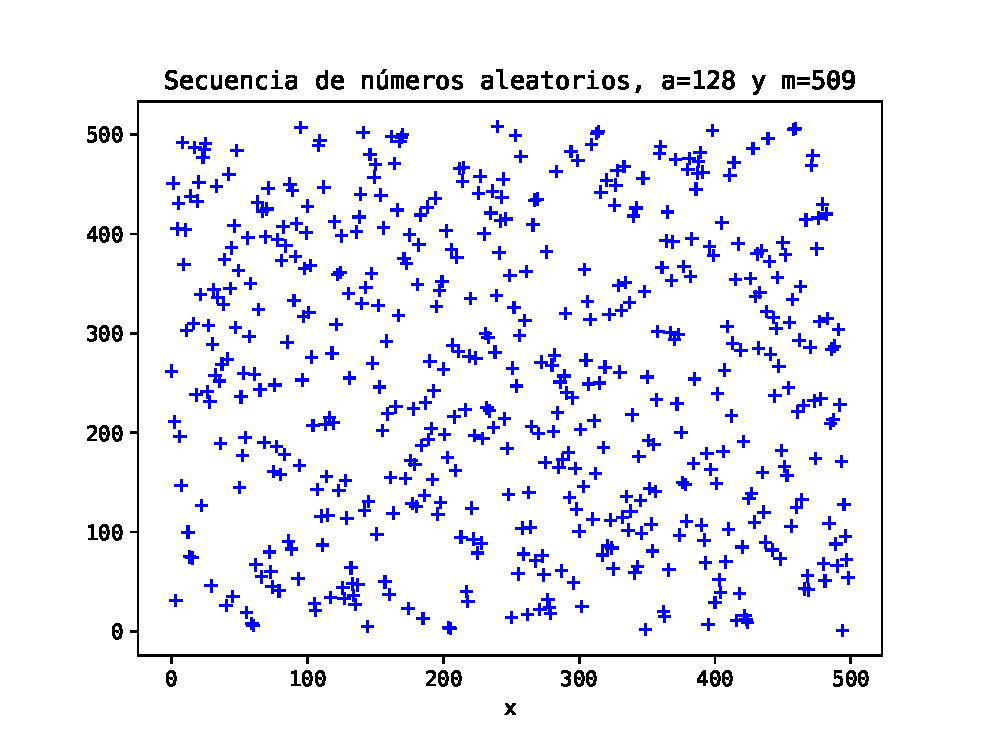
\includegraphics[scale=0.6]{Imagenes/Secuencia_aleatoria_01.eps}
\end{figure}
\end{frame}
\begin{frame}[fragile]
\frametitle{Distribución de números aleatorios (2/2)}
\begin{figure}
 \centering
 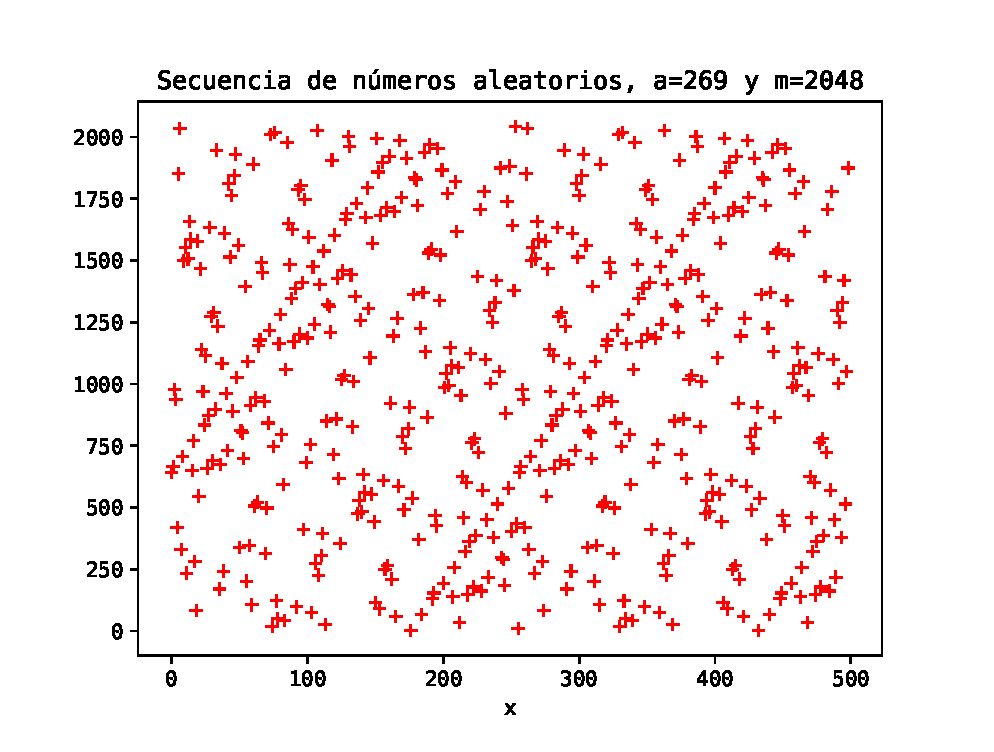
\includegraphics[scale=0.6]{Imagenes/Secuencia_aleatoria_02.eps}
\end{figure}
\end{frame}
\begin{frame}
\frametitle{Pregunta}
De las dos gráficas obtenidas: ¿Darías por hecho que las secuencias son aleatorios? ¿Hay algún patrón en la distribución de puntos?
\end{frame}
\subsection{La librería \texttt{random}}
\begin{frame}
\frametitle{La librería \texttt{random}}
Este módulo implementa generadores de números pseudoaleatorios para diversas distribuciones.
\\
\bigskip
Para números enteros, hay selección uniforme de un rango. Para las secuencias, hay una selección uniforme de un elemento aleatorio, una función para generar una permutación aleatoria de una lista \emph{in situ} y una función para el muestreo aleatorio sin reemplazo.
\end{frame}
\begin{frame}
\frametitle{La librería \texttt{random}}
Casi todas las funciones de la librería dependen de la función básica \funcionazul{random ()}, que genera un número flotante aleatorio de manera uniforme en el rango semiabierto $[0.0, 1.0)$
\end{frame}
\begin{frame}
\frametitle{La librería \texttt{random}}
En \python{} se usa el algoritmo \textoazul{Mersenne Twister} como generador central.
\\
\bigskip
Genera números flotantes de precisión de $53$ bits y tiene un período de $2^{19937}-1$.
\end{frame}
\begin{frame}
\frametitle{Alcance del generador en \texttt{random}}
El algoritmo \textoazul{Mersenne Twister} es uno de los generadores de números aleatorios más probados que existen.
\\
\bigskip
Sin embargo, al ser completamente determinista, no es adecuado para todos los propósitos, y es completamente inadecuado para fines criptográficos.
\end{frame}
\begin{frame}
\frametitle{Funciones importantes}
Dentro de la librería \funcionazul{random} existen distintas funciones que podremos utilizar, basta con revisar la documentación disponible, para identificar los parámetros y la respuesta que devuelve.
\end{frame}
\begin{frame}
\frametitle{Funciones importantes}
Mencionaremos dos funciones:
\setbeamercolor{item projected}{bg=green!70!black,fg=white}
\setbeamertemplate{enumerate items}[circle]
\begin{enumerate}[<+->]
\item \funcionazul{random.seed(a=None)}. Inicializa el generador de números aleatorios. Si no se especifica el valor de $a$, se utiliza el reloj del sistema. En caso de que $a$ sea un entero, se utiliza directamente.
\item \funcionazul{random.random()}. Devuelve un número de punto flotante en el rango $[0.0, 1.0)$.
\end{enumerate}
\end{frame}
\begin{frame}
\frametitle{Usando \texttt{seed} y \texttt{random}}
En el siguiente ejemplo se ejecuta el código para generar una secuencia de números aleatorios con la función \funcionazul{random}, que toma la semilla de la función \funcionazul{seed}.
\\
\bigskip
Al cerrar la ventana de la gráfica, se vuelve a ejecutar el código y veremos que la secuencia de números ya es distinta, debido a que se modificó la hora del sistema.
\end{frame}
\begin{frame}[allowframebreaks, fragile]
\frametitle{Ejemplo con \texttt{seed} y \texttt{random}}
\begin{lstlisting}[caption=Ejemplo de uso de las funciones del módulo \texttt{random}, style=codigopython]
import random

def generaazar(muestra, semilla=None):
    def arreglo(lista):
        for i in range(muestra):
            nuevoValor = random.random()
            lista.append(nuevoValor)
        return lista
    
    random.seed(semilla)    
    listaA_1_B = []
    listaA_2_B = []
    valoresRandomX = arreglo(listaA_1_B)
    valoresRandomY = arreglo(listaA_2_B)
    return valoresRandomX, valoresRandomY

muestra = 500
xA_1_B, yA_1_B = generaazar(muestra)
\end{lstlisting}
\end{frame}
\begin{frame}
\frametitle{Gráficas obtenidas 1/2}
\begin{figure}[h!]
  \centering
  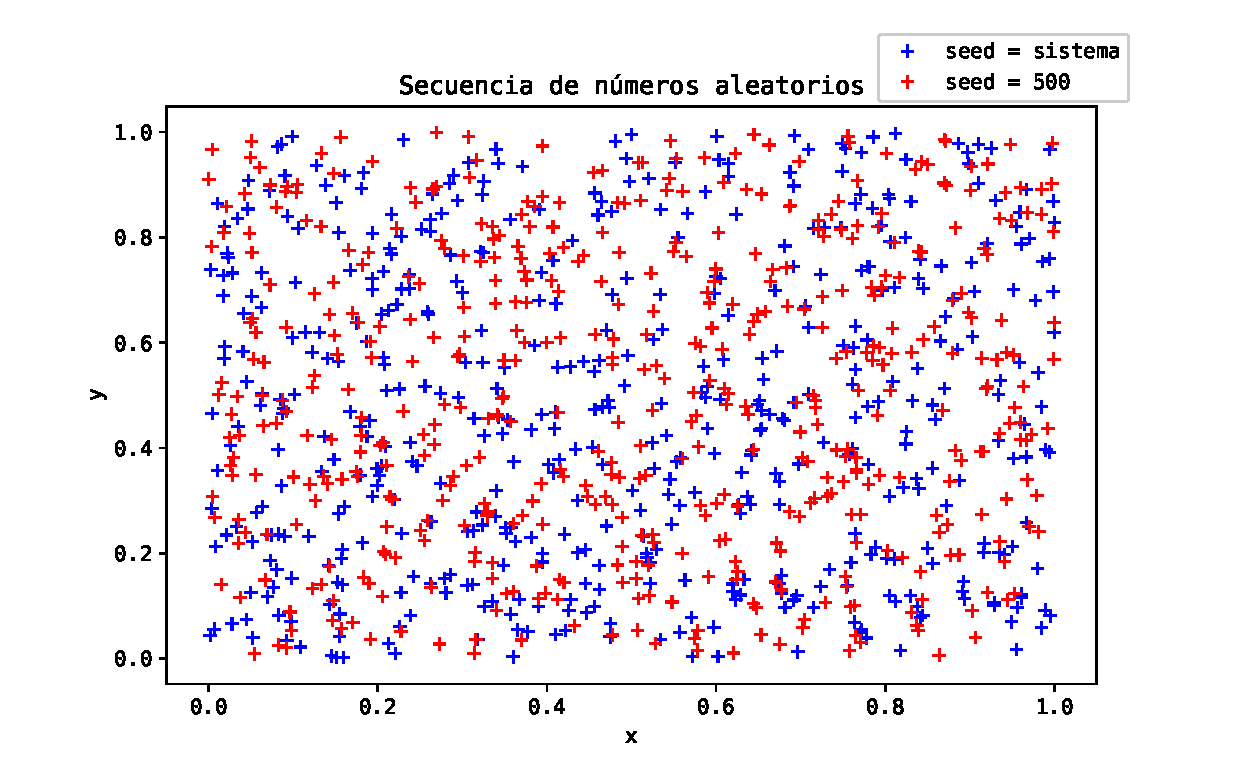
\includegraphics[scale=0.5]{Imagenes/Secuencia_aleatoria_03.eps}
\end{figure}
\end{frame}
\begin{frame}
\frametitle{Gráficas obtenidas 2/2}
\begin{figure}[h!]
  \centering
  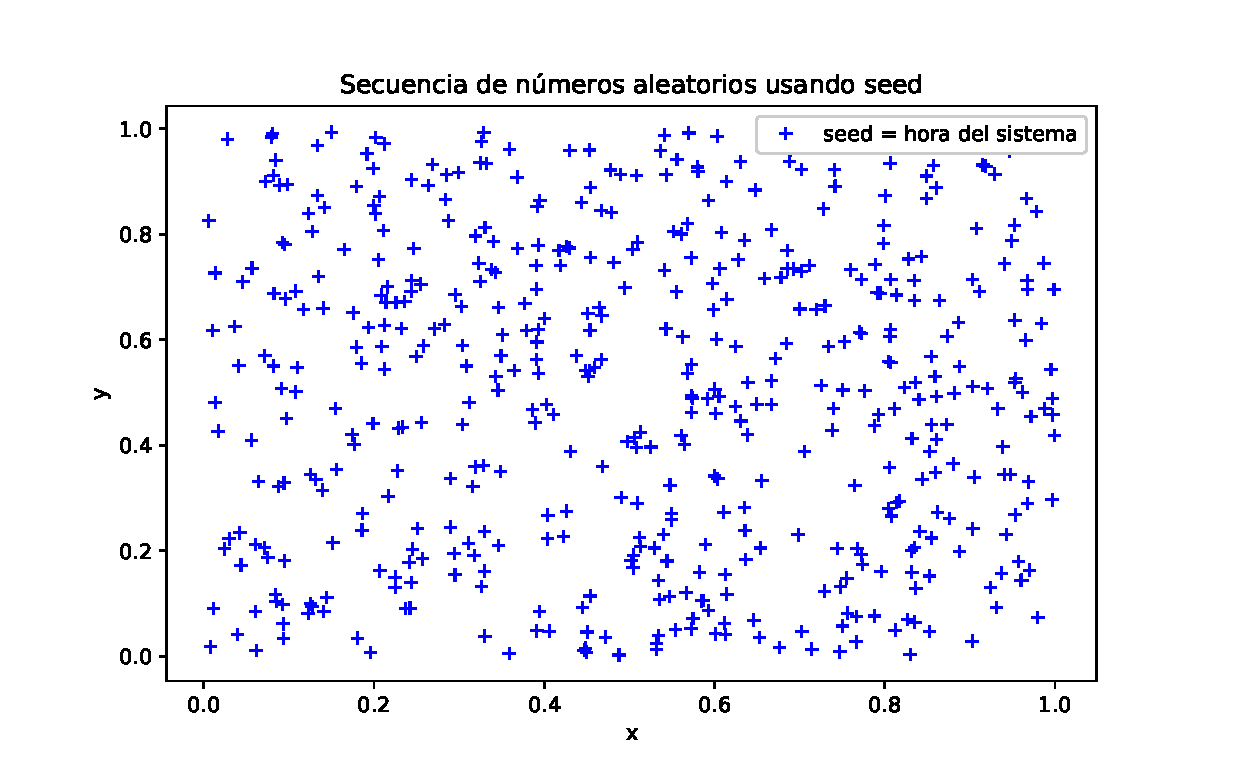
\includegraphics[scale=0.5]{Imagenes/Secuencia_aleatoria_04.eps}
\end{figure}
\end{frame}
\begin{frame}
\frametitle{Sobre las gráficas}
Las gráficas anteriores se obtuvieron con el mismo código, habiendo un cambio en el reloj del equipo, entonces la distribución de números aleatorios se modifica.
\end{frame}
\begin{frame}
\frametitle{Ejemplo con \texttt{random.seed(a)}}
Haremos un ejercicio en donde se van a generar dos secuencias de números con la función \funcionazul{random.seed(a)}, cambiaremos el valor de la semilla y vamos a comparar los resultados en una gráfica.
\\
\bigskip
Vamos a agregar una línea de código, la rutina de graficación habrá que implementarla.
\end{frame}
\begin{frame}[plain, allowframebreaks, fragile]
\frametitle{Código usando \texttt{seed()}}
\begin{lstlisting}[caption=Código con números generados con la hora del sistema y con semillas, style=codigopython]
xA_2_B, yA_2_B = generaazar(muestra, 500)
\end{lstlisting}
\end{frame}
\begin{frame}[fragile]
\frametitle{Gráfica obtenida}
\begin{figure}
 \centering
 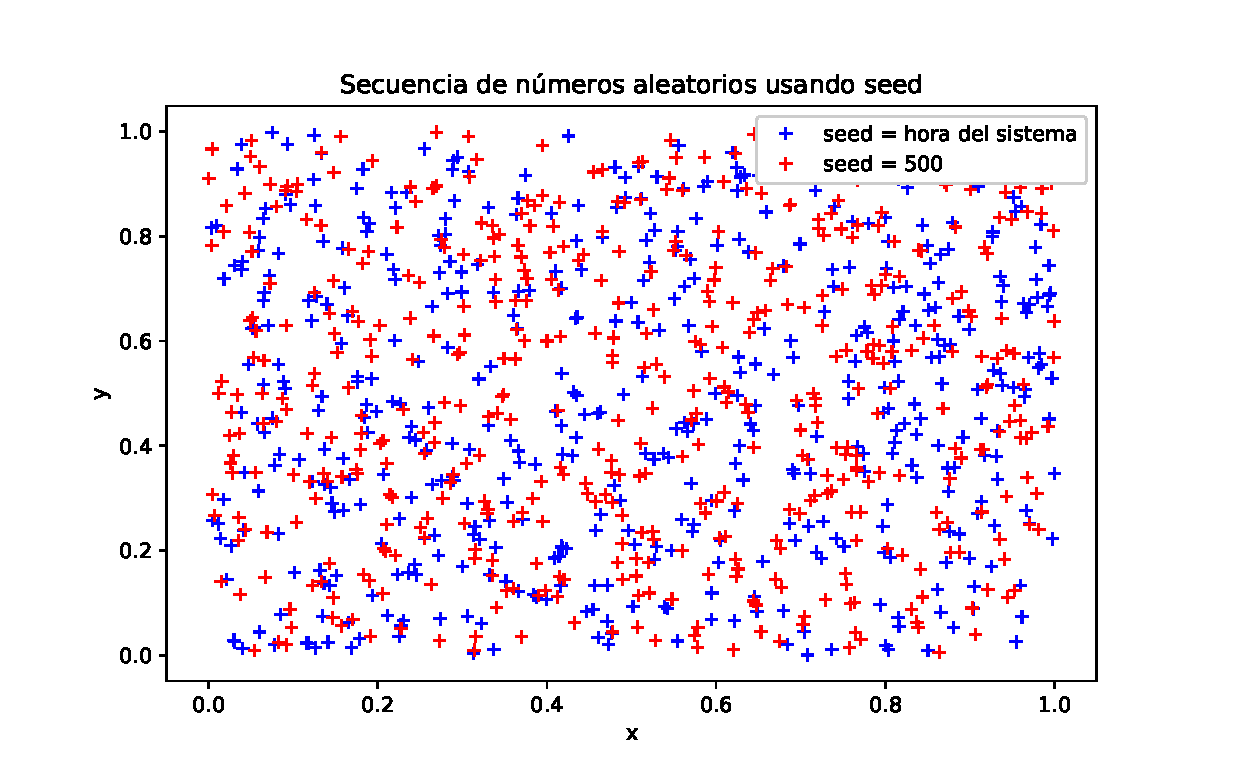
\includegraphics[scale=0.5]{Imagenes/Secuencia_aleatoria_05.eps}
\end{figure}
\end{frame}
% \section{La aguja de Buffon}
% \frame{\tableofcontents[currentsection, hideothersubsections]}
% \subsection{Planteamiento}
% \begin{frame}
% \frametitle{La aguja de Buffon}
% Resulta que $\pi$ también desempeña un papel importante en un experimento llamado \enquote{el problema de la aguja de Buffon}.
% \\
% \bigskip
% \pause
% El cual determina la probabilidad de que una aguja de longitud $\ell$, arrojada aleatoriamente aterrice en medio o atravesando una serie de líneas paralelas en el suelo.
% \end{frame}
% \begin{frame}
% \frametitle{El lanzamiento de la aguja}
% \begin{figure}
% 	\centering
% 	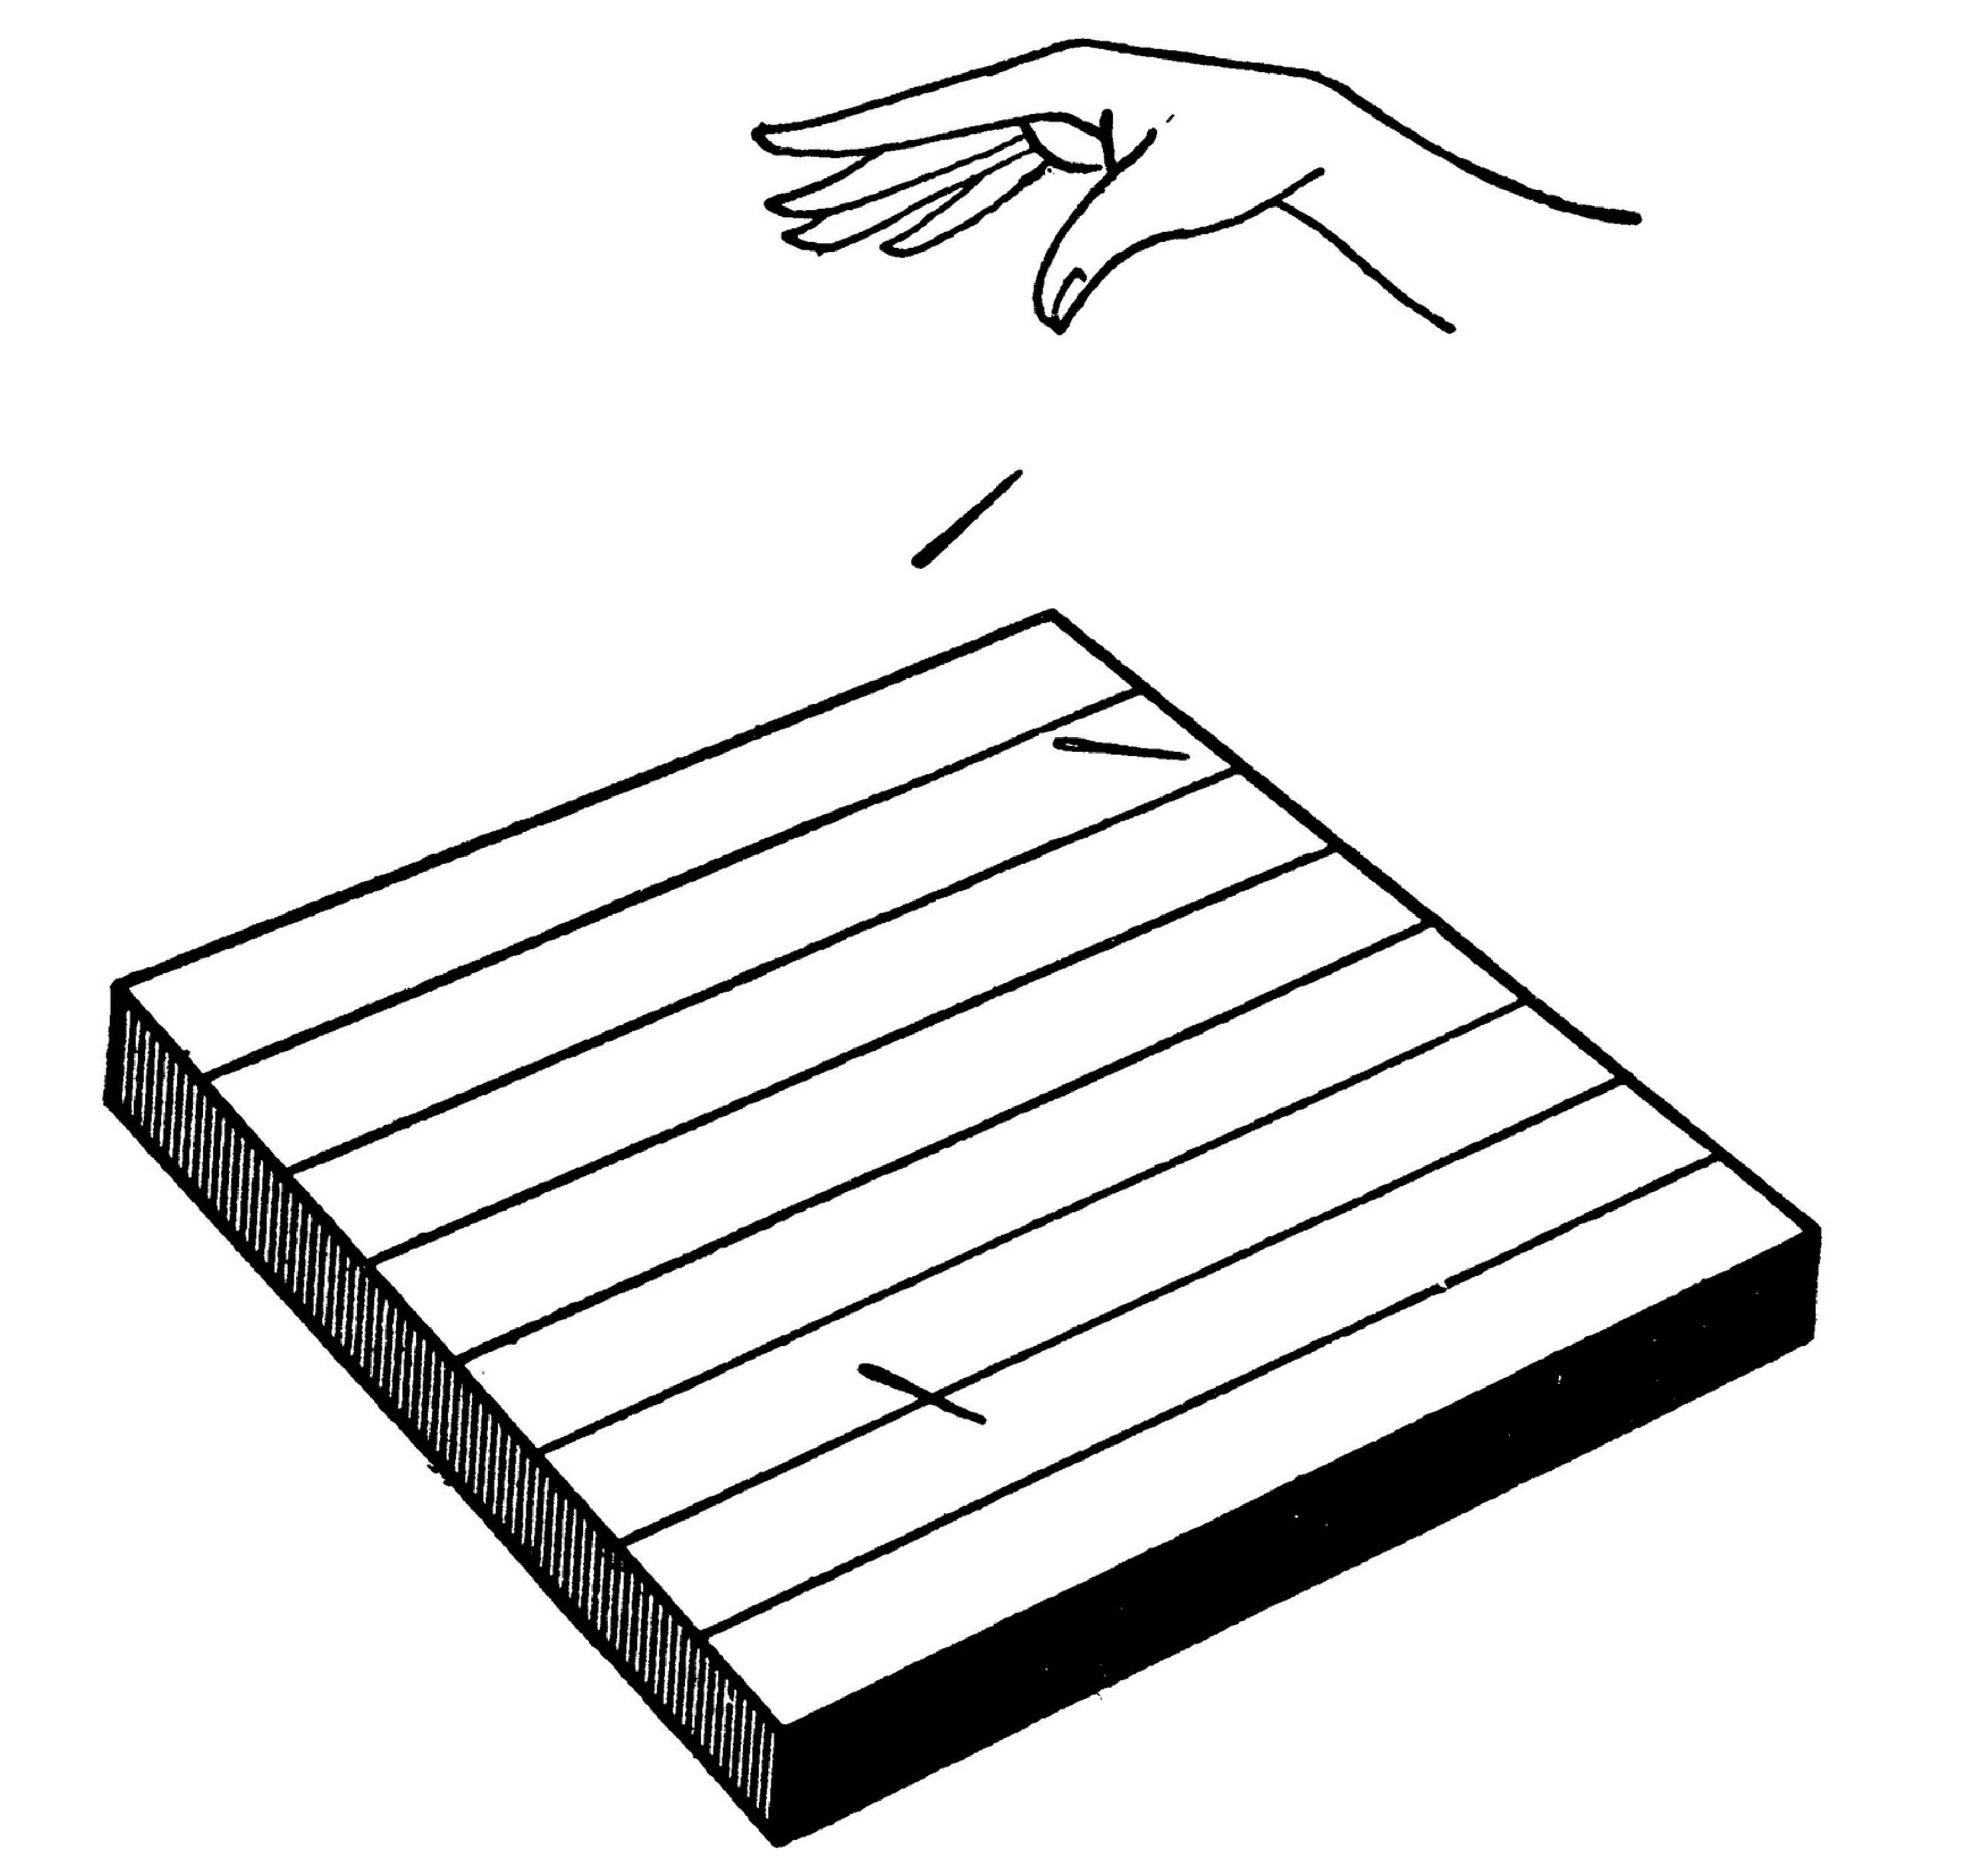
\includegraphics[scale=0.10]{Imagenes/aguja-de-buffon.eps}
% \end{figure}
% La separación entre las líneas es constante.
% \end{frame}
% \begin{frame}
% \frametitle{La aguja de Buffon}
% Resulta que si la distancia entre las líneas paralelas es la misma que la longitud $\ell$ de la aguja lanzada, el número de veces que la aguja cae atravesando las líneas (luego de un gran número de lanzamientos), nos servirá para calcular el valor de $\pi$.
% \end{frame}
% \subsection{Aproximación al valor de pi}
% \begin{frame}
% \frametitle{Aproximación al valor de $\pi$}
% De esa manera: 
% \begin{align*}
% \pi = \dfrac {2 \, N}{A}
% \end{align*}
% siendo $N$ el número total de intentos y $A$ el número de veces que la aguja ha cruzado alguna línea.
% \end{frame}
% \begin{frame}
% \frametitle{Primer problema de tarea}
% Considera el caso en el que la longitud de la aguja es igual a la separación entre las rayas, es decir $\ell = h$.
% \\
% \bigskip
% Si la aguja cruza una línea de manera oblicua, es decir, existe un ángulo de inclinación con respecto a la línea, puedes deducir la relación a partir de la \enquote{función} que describe el caso de las agujas que tocan las líneas.
% \end{frame}
% \begin{frame}
% \frametitle{Segundo problema de tarea}
% Una vez que has deducido el problema, implementa en python un programa que calcule el valor aproximado de $\pi$, a partir del número de lanzamientos, y el número de agujas que cruzan una línea.
% \\
% \bigskip
% En las siguientes gráficas verás los resultados cuando se realiza el lanzamiento de $10^{2}, 10^{3}, 10^{4}, 10^{5}, 10^{6}$ agujas.
% \end{frame}
% % \begin{frame}
% % \frametitle{Configuración para el problema de la aguja}
% % \begin{figure}[fragile]
% % \begin{tikzpicture}{font=\small}
% % 	\draw [thick] (0, 0) -- (7,0);
% % 	\draw [thick] (0, 4) -- (7,4);
% % 	\draw [<->] (1,0) -- node[left] {Distancia entre líneas = 1}(1, 4);
% % \end{tikzpicture}
% % \end{figure}
% % \end{frame}
% \begin{frame}
% \frametitle{Solución con python}
% \begin{figure}
%  \centering
%  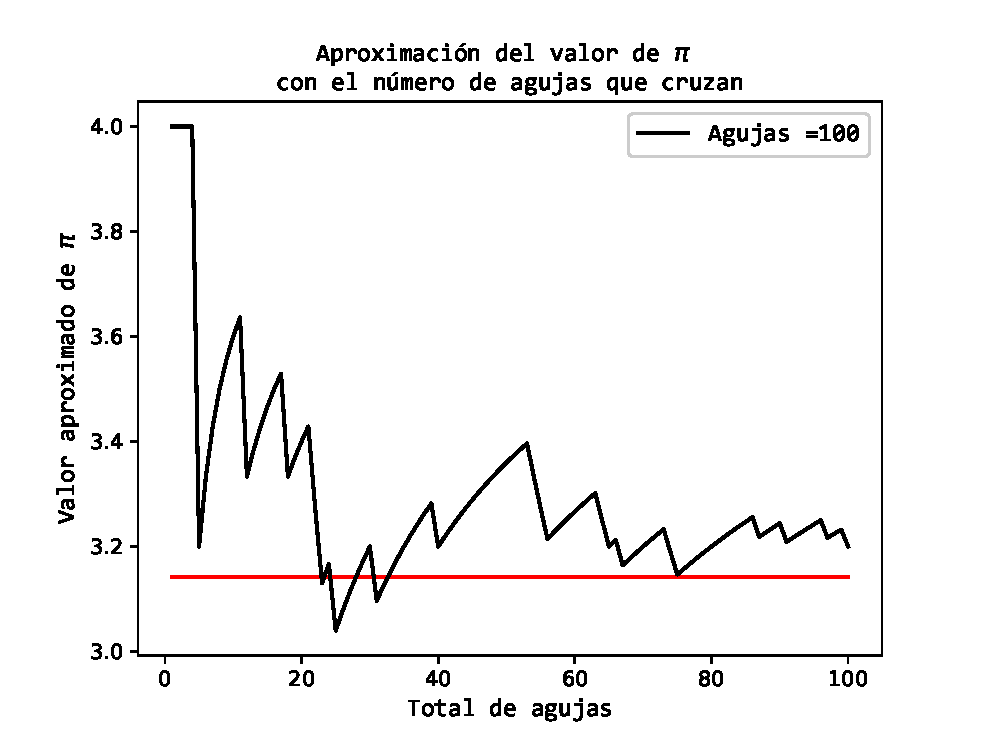
\includegraphics[scale=0.6]{aproximacionPi_100.eps}
% \end{figure}
% \end{frame}
% \begin{frame}
% \frametitle{Solución con python}
% \begin{figure}
%  \centering
%  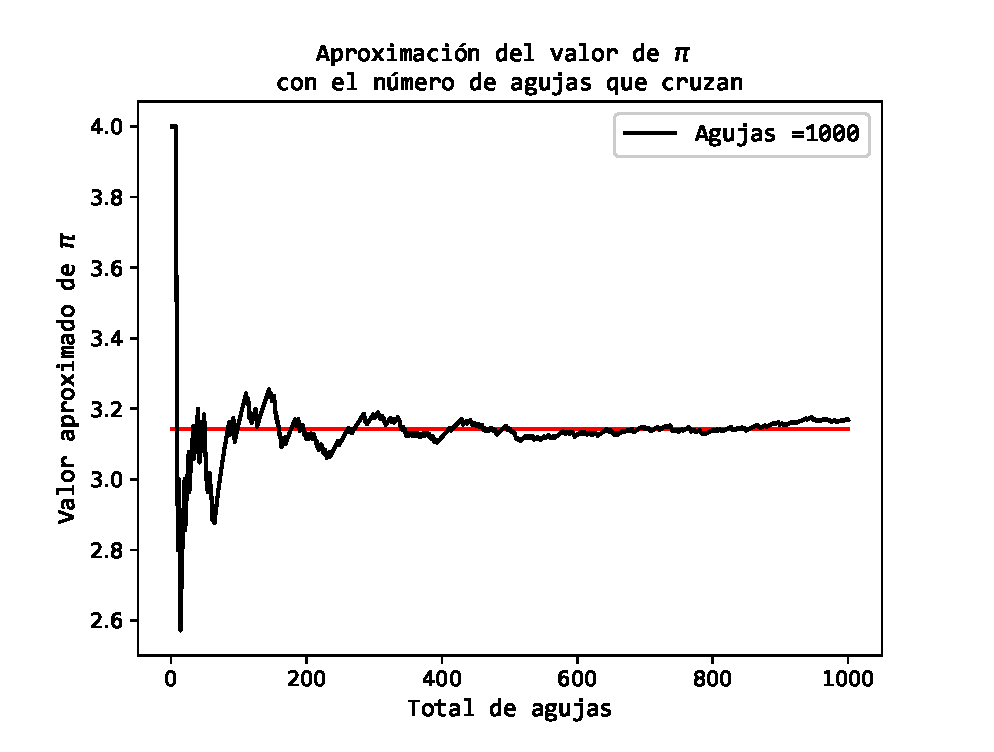
\includegraphics[scale=0.6]{aproximacionPi_1000.eps}
% \end{figure}
% \end{frame}
% \begin{frame}
% \frametitle{Solución con python}
% \begin{figure}
%  \centering
%  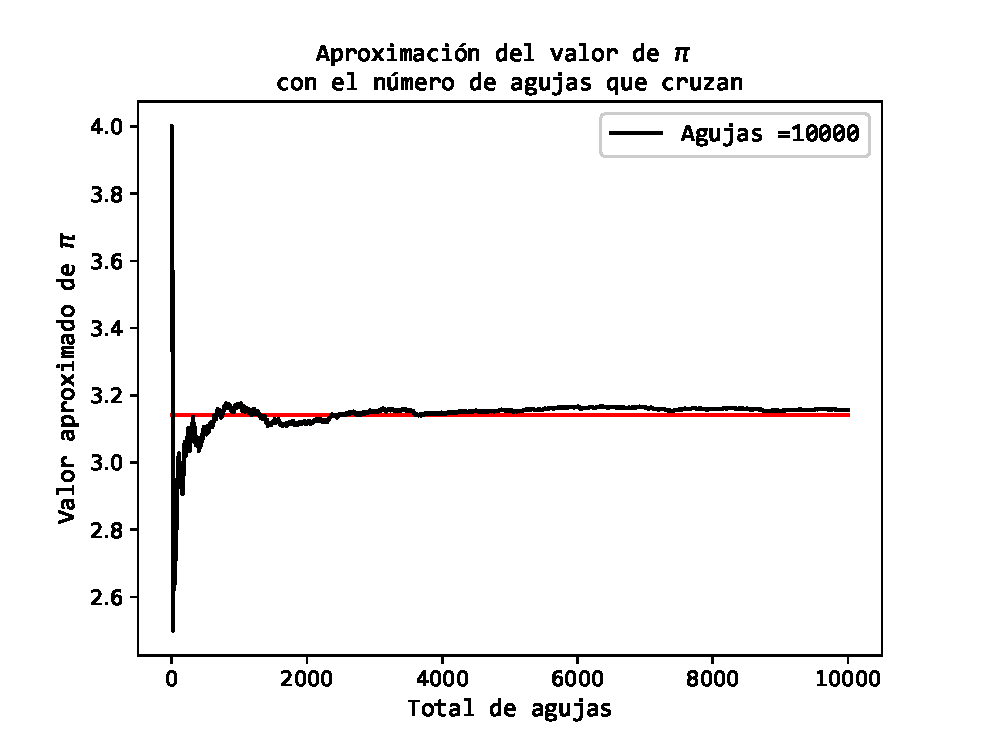
\includegraphics[scale=0.6]{aproximacionPi_10000.eps}
% \end{figure}
% \end{frame}
% \begin{frame}
% \frametitle{Solución con python}
% \begin{figure}
%  \centering
%  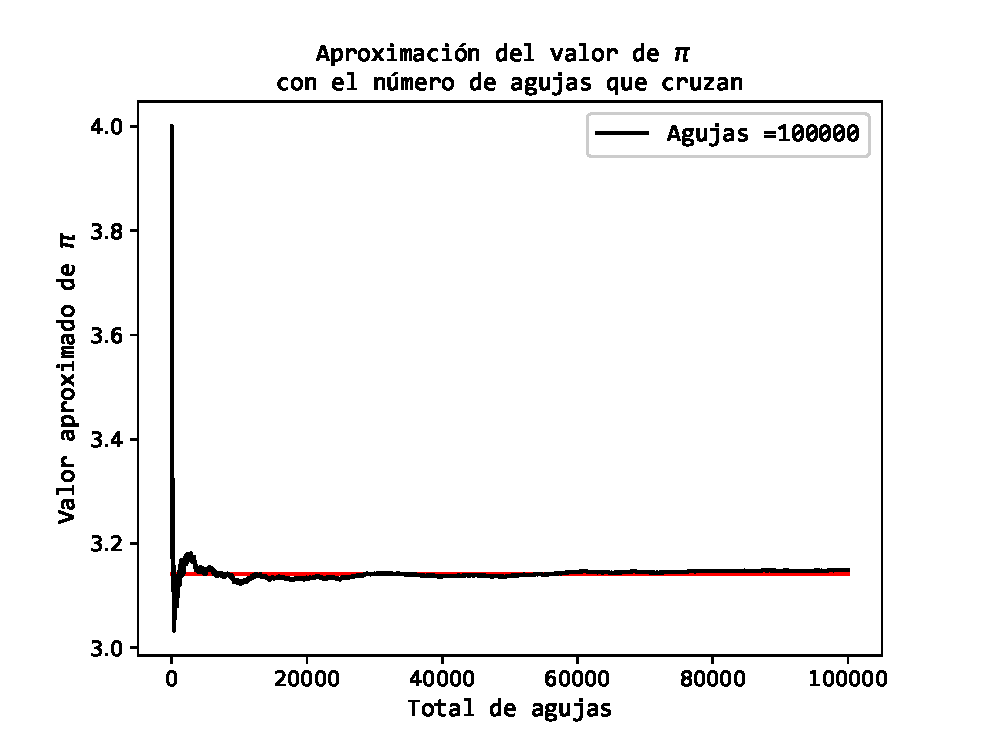
\includegraphics[scale=0.6]{aproximacionPi_100000.eps}
% \end{figure}
% \end{frame}
% \begin{frame}
% \frametitle{Solución con python}
% \begin{figure}
%  \centering
%  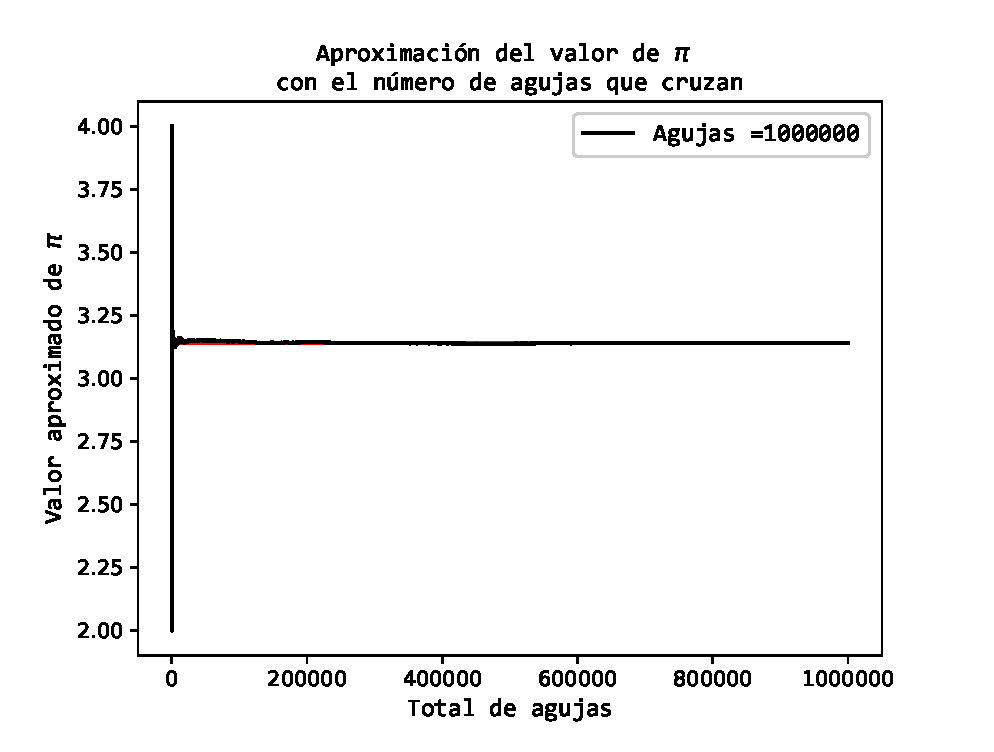
\includegraphics[scale=0.6]{aproximacionPi_1000000.eps}
% \end{figure}
% \end{frame}
%Referencia. Langtangen. A primer on scientific programming with pyhon. Chap. 8. Random
% numbers and simple games
\section{Integración Monte Carlo}
\frame{\tableofcontents[currentsection, hideothersubsections]}
\subsection{Definición}
\begin{frame}
\frametitle{Integración Monte Carlo}
Una de las primeras aplicaciones con el uso de números aleatorios ha sido el cálculo numérico de integrales, es decir, un problema no aleatorio (determinista).
\\
\bigskip
Veamos un primer método para calcular la siguiente integral
\begin{align*}
\int_{a}^{b} f(x) \; \dd{x}
\end{align*}
\end{frame}
\begin{frame}
\frametitle{Integración estándar Monte Carlo}
Sea $x_{1}, x_{2}, \ldots, x_{n}$ la secuencia de números aleatorios uniformemente distribuidos entre $a$ y $b$, puntos de un intervalo.
\\
\bigskip
Entonces
\begin{align}
(b - a) \; \dfrac{1}{n} \; \sum_{i=1}^{n} f(x_{i})
\label{eq:ecuacion_08_07}
\end{align}
\end{frame}
\subsection{Aproximación a la integral}
\begin{frame}
\frametitle{Aproximación a la integral}
Es una aproximación a la integral 
\begin{align}
\int_{a}^{b} f(x) \dd{x} 
\end{align}
Este método se denomina generalmente \emph{integración de Monte Carlo}.
\end{frame}
\begin{frame}
\frametitle{Aproximación a la integral}
Es fácil de interpretar la ec. (\ref{eq:ecuacion_08_07}): Un resultado bien conocido del cálculo es que la integral de una función $f$ sobre $[a, b]$ es igual al valor medio de $f$ sobre $[a, b]$ multiplicado por la longitud del intervalo, $(b - a)$.
\end{frame}
\begin{frame}
\frametitle{Aproximación a la integral}
Si aproximamos el valor medio de $f(x)$ por la media de $n$ evaluaciones de la función distribuidas al azar $f(x_{i})$, obtenemos el método de integración descrito.
\\
\bigskip
Podemos implementar la ec. (\ref{eq:ecuacion_08_07}) en una pequeña función de \python:
\end{frame}
\subsection{Estimando con \texttt{python}}
\begin{frame}[allowframebreaks, plain, fragile]
\frametitle{Estimado la integral con python}
\begin{lstlisting}[caption=Función para aproximar la integral, style=codigopython]
import random

def MCint(f, a, b, n):
    s = 0
    for i in range(n):
        x = random.uniform(a, b)
        s += f(x)
    I = (float(b-a)/n) * s
    return I
\end{lstlisting}
\end{frame}
\begin{frame}[fragile]
\frametitle{Versión más rápida del código}
Normalmente se necesita un valor de $n$ grande para obtener buenos resultados con este método, por lo que es útil contar con una versión vectorizada, que es más rápida que la función anterior:
\end{frame}
\begin{frame}[plain, fragile]
\frametitle{Versión más rápida del código}
\begin{lstlisting}[caption=Función vectorizada para la aproximación de la integral, style=codigopython]
import random
from numpy import *

def MCintvec(f, a, b, n):
    x = random.uniform(a, b, n)
    s = sum(f(x))
    I = (float(b-a)/n) * s
    return I
\end{lstlisting}
\end{frame}
\begin{frame}
\frametitle{Ejemplo}
Vamos a probar el método de integración de Monte Carlo en una función simple, sea $f(x) = 2 + 3 \: x$, y calculemos la integral en $[1, 2]$.
\\
\bigskip
La mayoría de los otros métodos de integración numérica resolverán exactamente esa función lineal, independientemente del número de evaluaciones de la función.
\end{frame}
\begin{frame}
\frametitle{Ejemplo}
Pero este no es el caso de la integración de Monte Carlo. 
\\
\bigskip
Sería interesante ver cómo la calidad de la aproximación de Monte Carlo se incrementa, conforme crece el valor de $n$.
\end{frame}
\begin{frame}
\frametitle{Ejemplo}
Para graficar la evolución de la aproximación con la integral, debemos almacenar los valores intermedios $I$, por lo que debemos de modificar el código:
\end{frame}
\begin{frame}[allowframebreaks, plain, fragile]
\begin{lstlisting}[caption=Código para el ejercicio, style=codigopython]
def MCintA_2_B(f, a, b, n):
    # se guardan las aproximaciones intermedias de la integral en el arreglo I,
    # donde I[k-1] es k veces la funcion evaluada
    s = 0

    I = np.zeros(n)

    for k in range(1, n+1):
        x = random.uniform(a, b)
        s += f(x)
        I[k-1] = (float(b-a)/k) * s
    return I
\end{lstlisting}
\end{frame}
\begin{frame}
\frametitle{Consideraciones para la solución}
Toma en cuenta que hacemos que $k$ vaya de $1$ a $n$ mientras que los índices en $I$, como de costumbre, van de $0$ a $n-1$.
\end{frame}
\begin{frame}
\frametitle{Consideraciones para la solución}
Dado que $n$ puede ser muy grande, el arreglo $I$ puede consumir más memoria de lo que tenemos disponible en la computadora.
\\
\bigskip
Por lo tanto, decidimos almacenar sólo cada $N$ valores de la aproximación. El determinar si un valor debe ser almacenado o no puede ser calculado por la función \texttt{mod}:
\end{frame}
\begin{frame}[plain, fragile]
\frametitle{Consideraciones para la solución}
\begin{lstlisting}[caption=Almacenamiento de valores, style=codigopython]
for k in range(1, n+1):
    if k % N == 0:
    	#se guarda
\end{lstlisting}
Es decir, cada vez que $k$ se divide $N$ sin ningún residuo, almacenamos el valor.
\end{frame}
\begin{frame}[plain, allowframebreaks, fragile]
\frametitle{La función completa sería:}
\begin{lstlisting}[caption=Código completo para el ejercicio, style=codigopython]
def MCintA_3_B(f, a, b, n, N=100):
    s = 0
    Ivalores = []
    kvalores = []
    
    for k in range(1, n+1):
        x = random.uniform(a, b)
        s += f(x)
        if k % N == 0:
            I = (float(b-a)/k) * s
            Ivalores.append(I)
            kvalores.append(k)
    
    return k_valores, I_valores
\end{lstlisting}
\end{frame}
\begin{frame}[plain, fragile]
\frametitle{Estimación del error}
Ahora podemos revisar el error que se genera al usar la función:
\begin{lstlisting}[caption=Estimación del error del procedimiento, style=codigopython]
def fA_1_B(x):
    return 2 + 3*x

k, I = MCintA_3_B(fA_1_B, 1, 2, 1000000, N=10000)
error = 6.5 - np.array(I)
\end{lstlisting}
\end{frame}
\begin{frame}
\frametitle{Agregar rutina de graficación}
Como en otras ocasiones, hay que incluir una rutina de graficación para obtener el resultado que se verá en la siguiente diapositiva. 
\end{frame}
\begin{frame}[fragile]
\frametitle{Gráfica del error vs $N$}
\begin{figure}
	\centering
	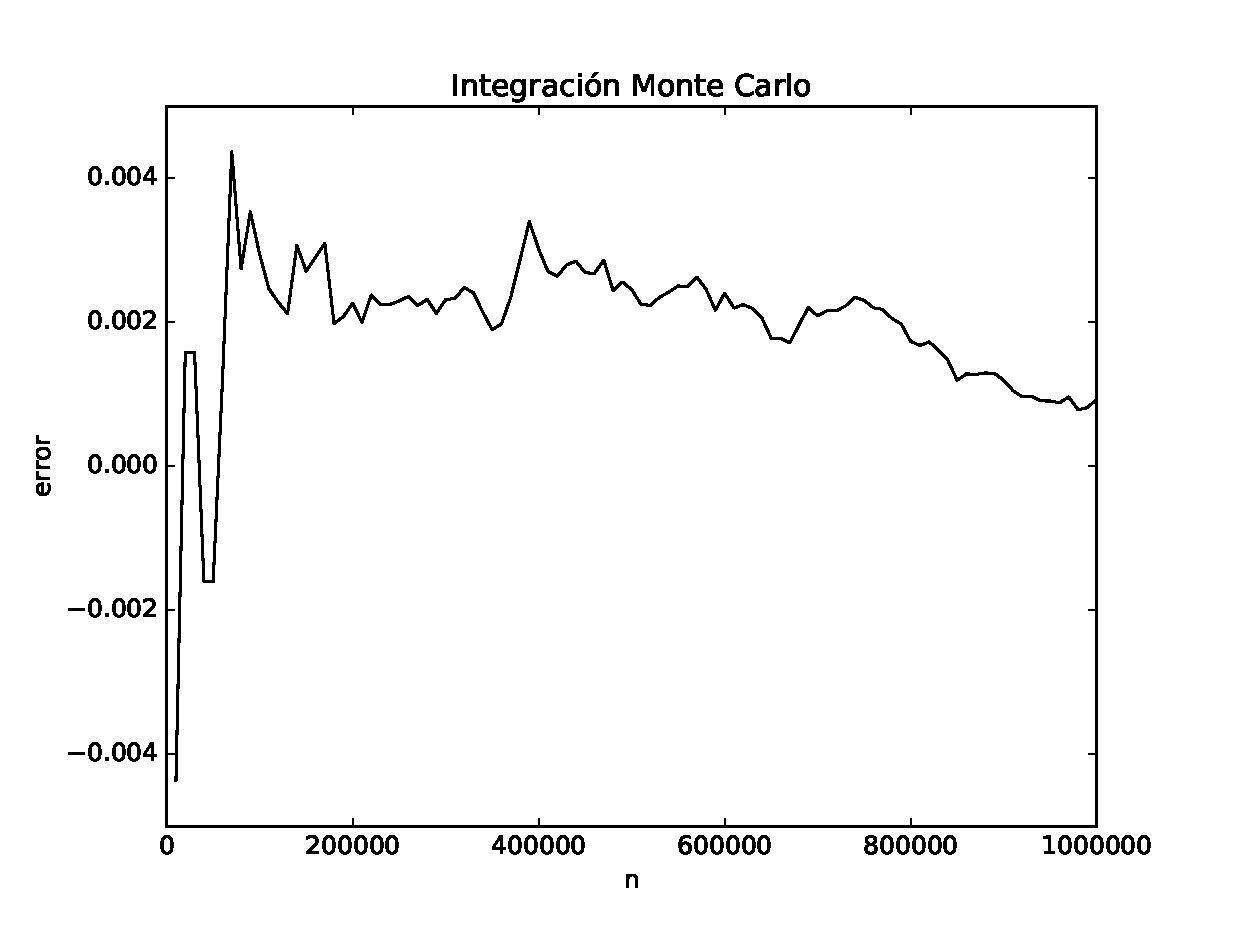
\includegraphics[scale=0.5]{Imagenes/integracionMC01.eps}
	\caption{Convergencia de la integración de Monte Carlo para $f(x)$}
\end{figure}
\end{frame}
\begin{frame}
\frametitle{Velocidad de convergencia}
Para funciones de una variable, el método (\ref{eq:ecuacion_08_07}) requiere de muchos puntos y es ineficiente comparado con otras reglas de integración.
\\
\bigskip
La mayoría de las reglas de integración tienen un error que se reduce mientras se incrementa $n$, normalmente de la manera $n^{-r}$ para un $r>0$.
\end{frame}
\begin{frame}
\frametitle{Velocidad de convergencia}
Para la regla del trapecio, $r = 2$, mientras que para la integración de Monte Carlo $r = 1/2$
\\
\bigskip
Esto significa que este método converge muy lentamente en comparación con la regla del trapecio.
\end{frame}
\subsection{Integración en varias variables}
\begin{frame}
\frametitle{Integración en varias variables}
Sin embargo, para funciones de varias variables, la integración de Monte Carlo en espacios de dimensiones mayores supera completamente a métodos como la regla del trapecio y la regla de Simpson.
\end{frame}
\begin{frame}
\frametitle{Mejoras para el cálculo de la integral}
Existen diferentes maneras de mejorar el rendimiento de la ec. (\ref{eq:ecuacion_08_07}), básicamente por ser \enquote{aplicados} al momento de graficar los números aleatorios, conocidas como \emph{técnicas de reducción de la varianza}.
\end{frame}
\subsection{Calculando áreas con puntos aleatorios}
\begin{frame}
\frametitle{Calculando áreas con puntos aleatorios}
Pensemos en alguna región geométrica $G$ en el plano y una caja circundante $B$ con geometría $[x_{L}, x_{H}] \cp [y_{L}, y_{H}]$.
\\
\bigskip
Una forma de calcular el área de $G$ es dibujar $N$ puntos aleatorios dentro de $B$ y contar cuántos de ellos $M$, están dentro de $G$.
\end{frame}
\begin{frame}
\frametitle{Puntos dentro de la región}
El área de $G$ es entonces la fracción $M/N$ (fracción de $G$ en el área de $B$) veces el área de $B$, $(x_{H} - x_{L})(y_{H} - y_{L})$.
\end{frame}
\begin{frame}
\frametitle{Puntos dentro de la región}
Expresado de forma distinta, este método es una especie de juego de dardos en el que se cuentan los que caen dentro de $G$, si cada lanzamiento llega de manera uniforme dentro de $B$.
\end{frame}
\begin{frame}
\frametitle{Calculando una integral}
Veamos cómo será la expresión para calcular la integral
\begin{align*}
\int_{a}^{b} f(x) \: \dd{x}
\end{align*}
\pause
Como nota relevante, consideremos que esta integral es el área debajo de la curva $y = f(x)$ y sobre el eje $x$, entre $x = a$ y $x = b$.
\end{frame}
\begin{frame}
\frametitle{Calculando una integral}
Introducimos un rectángulo $B$, tal que
\begin{align*}
B = \{ (x, y) \vert : a \leq x \leq b, \hspace{0.3cm} 0 \leq y \leq m \}
\end{align*}
donde $m \leq \max_{x \in [a, b]} \; f(x)$
\end{frame}
\begin{frame}
\frametitle{Calculando una integral}
El algoritmo para calcular el área bajo la curva se basa en dibujar $N$ puntos aleatorios dentro de $B$ y contar cuántos de ellos, $M$, están por encima del eje $x$  y cuántos por debajo de la curva $y = f(x)$, como se aprecia en la siguiente figura:
\end{frame}
\begin{frame}
\frametitle{Método del dardo}
\begin{figure}
	\centering
	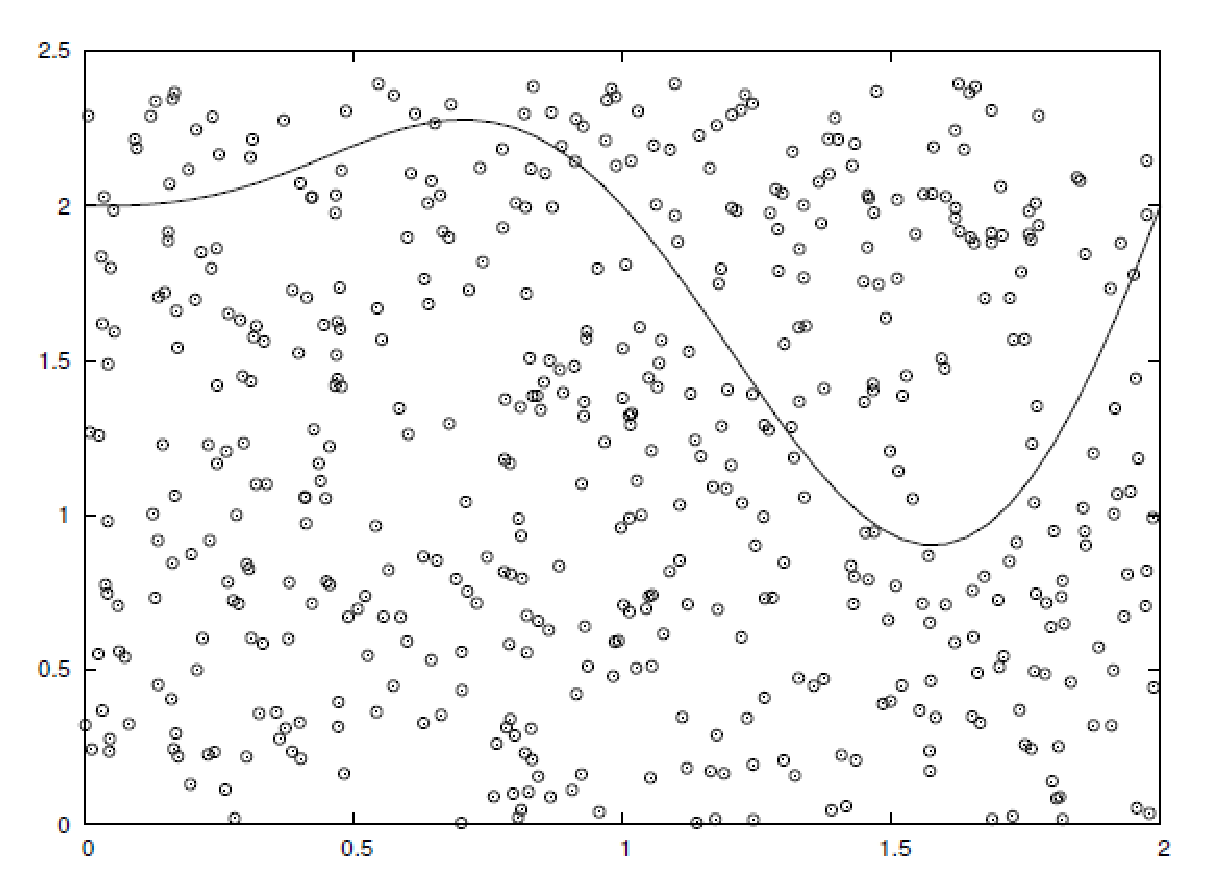
\includegraphics[scale=0.4]{Imagenes/integracionCaja.eps}
	\caption{\tiny{Cuando $M$ de $N$ puntos aleatorios en el rectángulo $[0, 2] \cp [0, 2.4]$ se encuentran bajo la curva, el área bajo la curva se estima como la fracción $M / N$ del área del rectángulo.}}
\end{figure}
\end{frame}
\begin{frame}
\frametitle{Valor de la integral}
El área o el valor de la integral se estima por la expresión
\begin{align*}
\dfrac{M}{N} \: m \: (b - a)
\end{align*}
\\
\bigskip
\pause
El código para el método del dardo sería:
\end{frame}
\begin{frame}[plain, fragile]
\frametitle{Código para la integral}
\begin{lstlisting}[caption=Código para el método del dardo, style=codigopython]
def MCint_area(f, a, b, n, m):
    porDebajo = 0 
    for i in range(n):
        x = random.uniform(a, b)
        y = random.uniform(0, m)
        if y <= f(x):
            porDebajo += 1
    area = porDebajo/float(n) * m * (b - a)
    
    return area
\end{lstlisting}
\end{frame}
\begin{frame}[fragile]
\frametitle{Consideración importante}
Toma en cuenta que este método opera con el doble de números aleatorios que el método anterior.
\\
\bigskip
Una implementación vectorizada del código es la siguiente:
\end{frame}
\begin{frame}[fragile]
\frametitle{Versión vectorizada}
\begin{lstlisting}[caption=Método del dardo en modo vectorizado, style=codigopython]
def MCint_area_vec(f, a, b, n, m):
    x = random.uniform(a, b, n)
    y = random.uniform(0, m, n)
    porDebajo = np.sum(y < f(x))
    area = porDebajo/float(n) * m * (b - a)
    
    return area
\end{lstlisting}
\end{frame}
\begin{frame}
\frametitle{Ventaja de la versión vectorizada}
Podemos ejecutar el código para un conjunto de 2 millones de números al azar, la versión de bucle sencillo no es tan lenta.
\\
\bigskip
\pause
Sin embargo, si necesita que la integración se repita muchas veces dentro de otro cálculo, puede ser importante la eficacia superior de la versión vectorizada.
\end{frame}
\begin{frame}[plain, allowframebreaks, fragile]
\frametitle{Función completa}
\begin{lstlisting}[caption=Función para el método del dardo, style=codigopython]
def MCintA_3_Barea(f, a, b, n, m, N=1000):
    Ivalores = []
    kvalores = []
    porDebajo = 0
    for k in range(1, n+1):
        x = random.uniform(a, b)
        y = random.uniform(0, m)
        if y <= f(x):
            porDebajo += 1
        area = porDebajo/float(k) * m * (b-a)
        if k % N == 0:
            I = area
            Ivalores.append(I)
            kvalores.append(2 * k)
    return kvalores, Ivalores
\end{lstlisting}
\end{frame}
\begin{frame}
\frametitle{Implementación del código}
Al contar con los elementos necesarios, podemos implementar el código completo para estimar el valor de la integral a partir de generar puntos aleatorios.
\\
\bigskip
Haremos una estimación del tiempo que tarda en resolverse el problema usando el bucle y la versión vectorizada.
\end{frame}
\begin{frame}
\frametitle{La librería \texttt{time}}
La librería \funcionazul{time} proporciona un conjunto de funciones para registrar el tiempo en el equipo de cómputo.
\\
\bigskip
Revisa la documentación de la librería, ya que \emph{tiene como punto particular el hecho de medir el tiempo a partir del 1 de enero de 1970}, al momento actual en el equipo.
\end{frame}
\begin{frame}
\frametitle{Para medir un intervalo}
Para el ejercicio que haremos, se requiere medir un intervalo de tiempo entre dos eventos, por lo que no es necesario hacer alguna conversión de tiempo.
\\
\bigskip
La función \funcionazul{time.process\_time()} hará el registro del tiempo en el equipo, para el intervalo, basta con que hagamos un segundo registro y tomar la diferencia entre éstos.
\end{frame}
\begin{frame}[plain, allowframebreaks, fragile]
\begin{lstlisting}[caption=Implementación del código, style=codigopython]
def fA_1_B(x):
    return 2 + 3 * x

a = 1; b = 2; n = 1000000; N = 10000; fmax = fA_1_B(b)

print('Metodo \t\t Integral')
print('-'*30)

tA_0_B = time.process_time()
print('Bucle \t\t {0:1.6f}'.format(MCint_area(fA_1_B, a, b, n, fmax)))

tA_1_B = time.process_time()
print('Vectorizacion \t {0:1.6f}'.format(MCint_area_vec(fA_1_B, a, b, n, fmax)))

tA_2_B = time.process_time()
fraccion = (tA_1_B-tA_0_B)/(tA_2_B-tA_1_B)

k, I = MCintA_3_B_area(fA_1_B, a, b, n, fmax, N)
print('Puntos abajo \t {0:1.6f}'.format(I[-1]))

print('fraccion puntos/bucle \t {0:1.8f}'.format(1/fraccion))

error = 6.5 - np.array(I)
\end{lstlisting}
\end{frame}
\begin{frame}
\frametitle{Resultado en la terminal}
El resultado obtenido es el siguente:
\begin{table}
\begin{tabular}{l c}
Método & Integral \\ \hline
Bucle & $6.501944$ \\ \hline
Vectorización & $6.492040$ \\ \hline
Puntos abajo & $6.501160$ \\ \hline
fraccion puntos/bucle & $0.04958678$ \\
\end{tabular}
\end{table}
\end{frame}
\begin{frame}[fragile]
\frametitle{Gráfica del error}
El error obtenido se presenta a continuación:
\begin{figure}[h!]
    \centering
    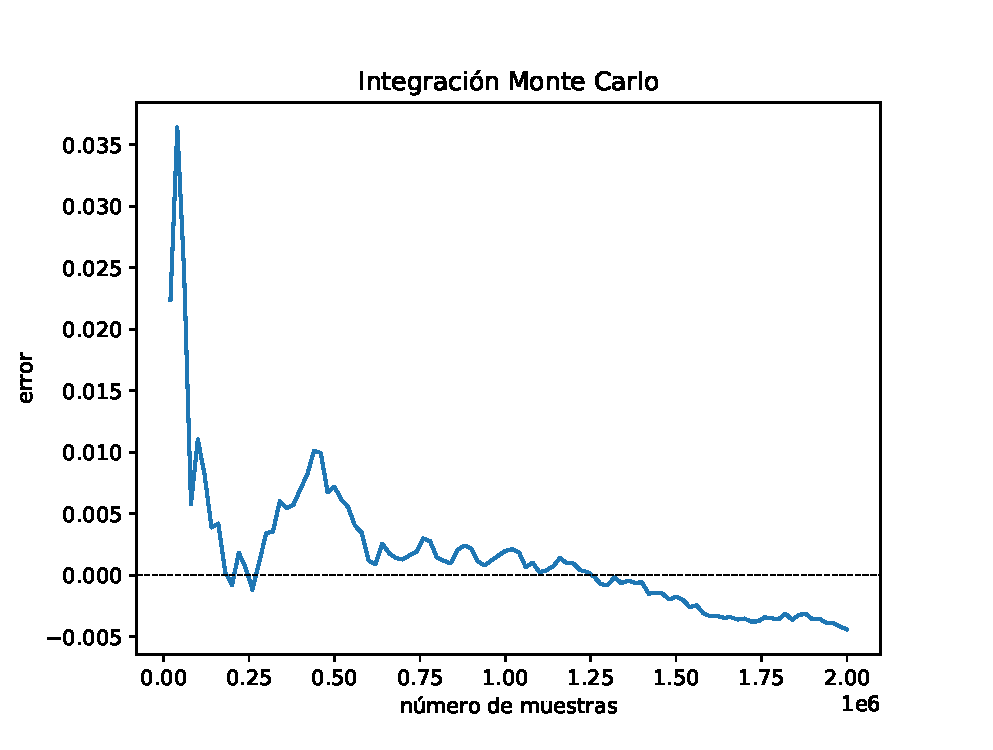
\includegraphics[scale=0.45]{Imagenes/integracion_area_01.eps}
    \caption{Comportamiento del error con el método del dardo.}
\end{figure}
\end{frame}
\begin{frame}
\frametitle{Graficando los puntos con el método}
A continuación se presenta una gráfica con los puntos aleatorios debajo de la función y por arriba de ésta, modificando el valor de $N$ para representar el método del dardo, se le ha puesto un color diferente para señalar cuando un punto está por debajo de la función y con otro color, cuando el punto está por arriba.
\end{frame}
\begin{frame}
\frametitle{Gráfica de la función en $[1, 2]$}
\begin{figure}[h!]
	\centering
	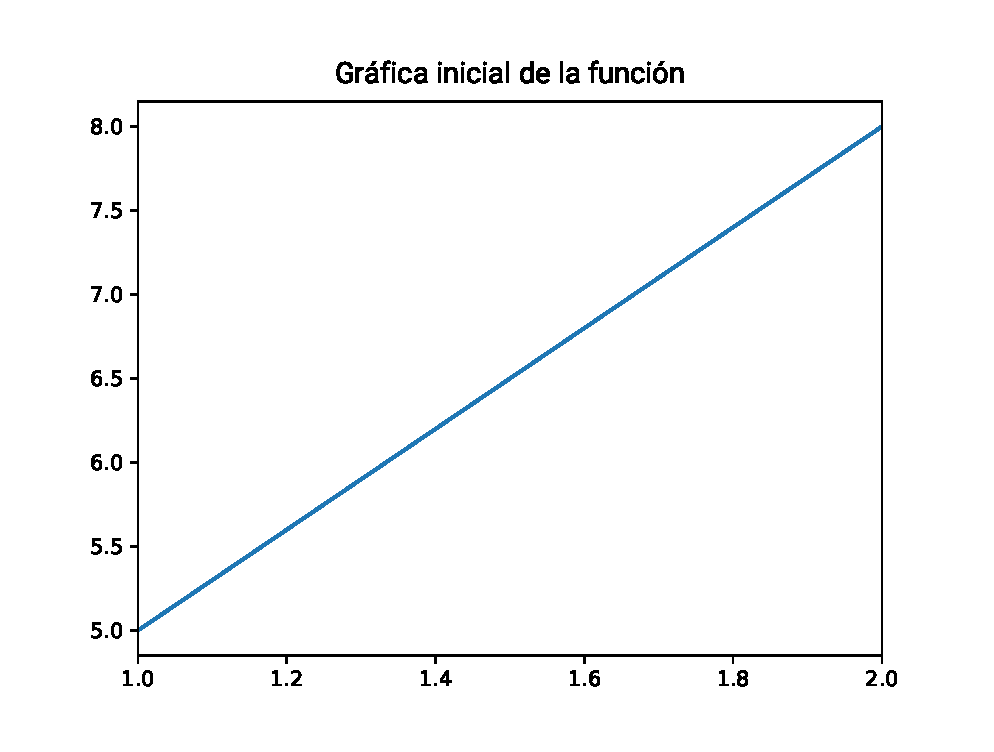
\includegraphics[scale=0.55]{Imagenes/area_puntos_01.eps}
    \caption{Función inicial.}
\end{figure}
\end{frame}
\begin{frame}
\frametitle{Gráfica al incluir puntos aleatorios}
\begin{figure}[h!]
    \centering
    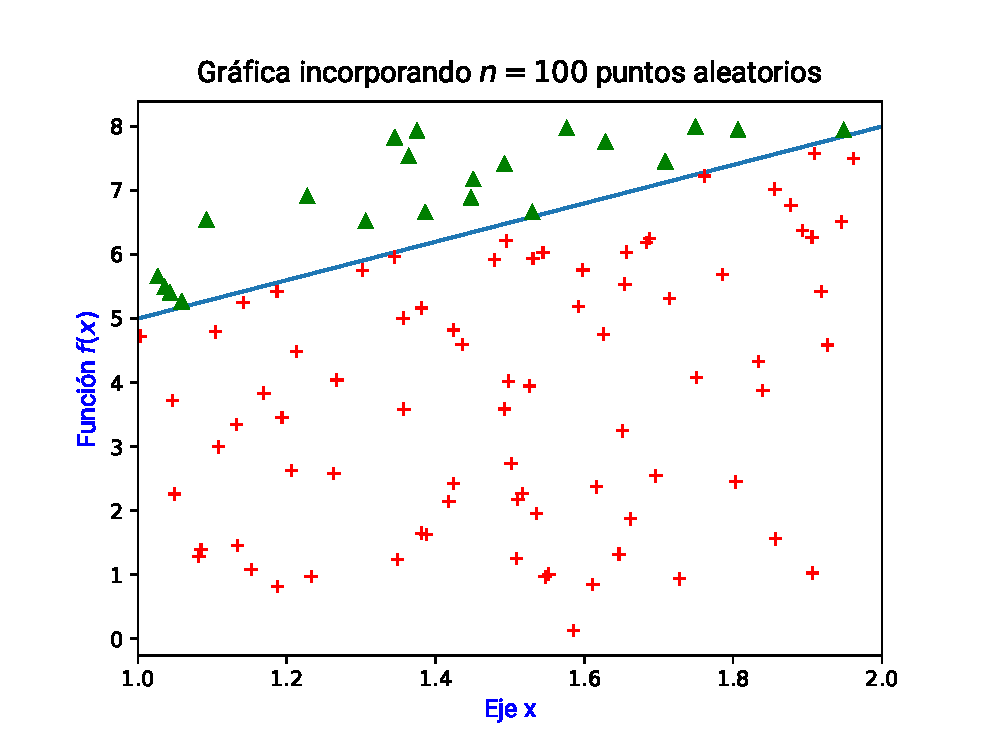
\includegraphics[scale=0.55]{Imagenes/area_puntos_02.eps}
    \caption{Puntos por arriba y por debajo de la función.}
\end{figure}
\end{frame}
\begin{frame}
\frametitle{Gráfica al incluir puntos aleatorios}
\begin{figure}[h!]
    \centering
    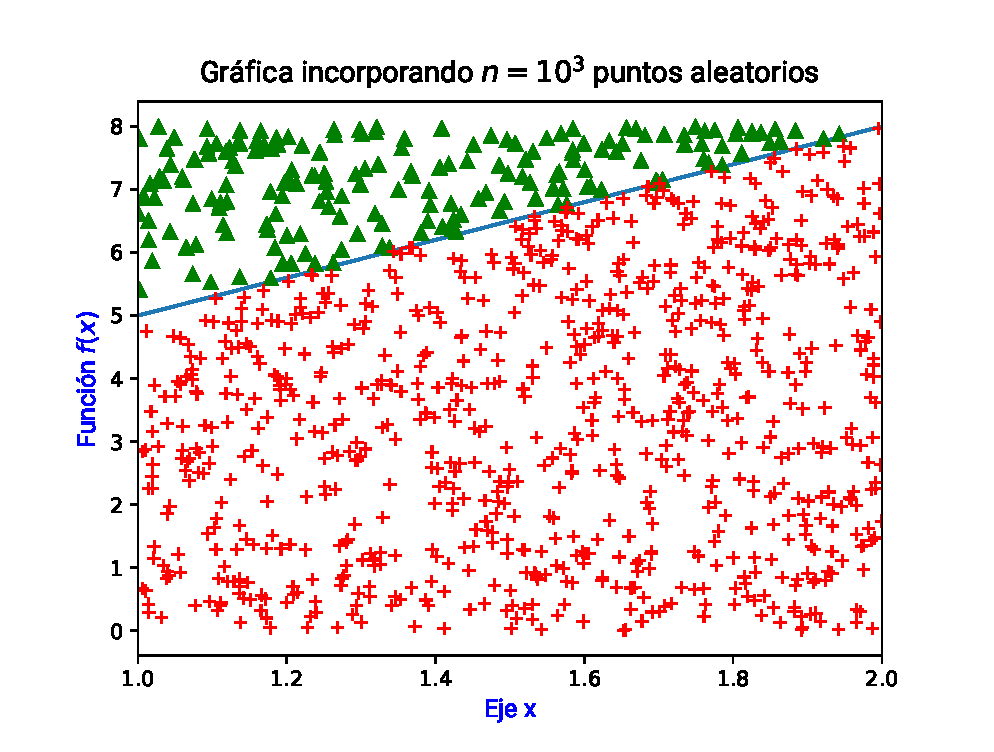
\includegraphics[scale=0.55]{Imagenes/area_puntos_03.eps}
    \caption{Se va saturando el área debajo de la curva.}
\end{figure}
\end{frame}
\begin{frame}
\frametitle{Gráfica al incluir puntos aleatorios}
\begin{figure}[h!]
    \centering
    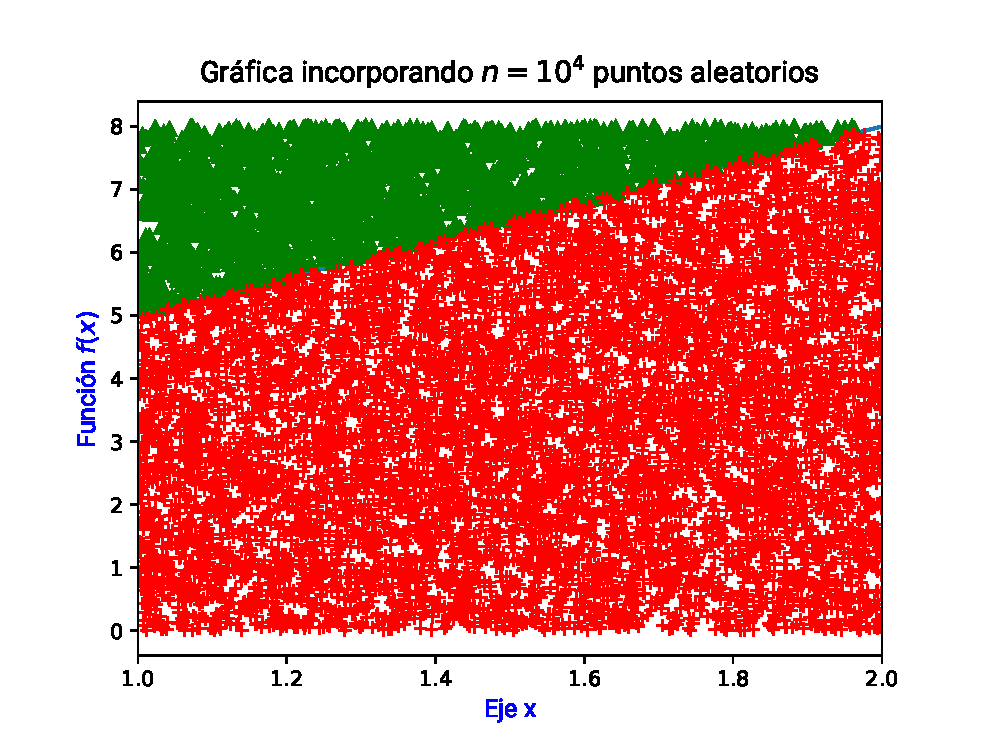
\includegraphics[scale=0.55]{Imagenes/area_puntos_04.eps}
    \caption{Casi se cubre el área debajo de la curva.}
\end{figure}
\end{frame}
\begin{frame}
\frametitle{Gráfica al incluir puntos aleatorios}
\begin{figure}[h!]
    \centering
    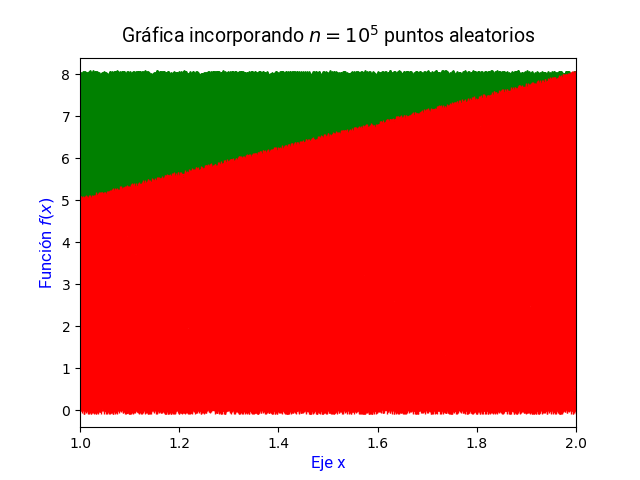
\includegraphics[scale=0.55]{Imagenes/area_puntos_05.png}
    \caption{Podríamos pensar que ya tenemos el valor de la integral.}
\end{figure}
\end{frame}
\begin{frame}
\frametitle{Gráfica al incluir puntos aleatorios}
\begin{figure}[h!]
    \centering
    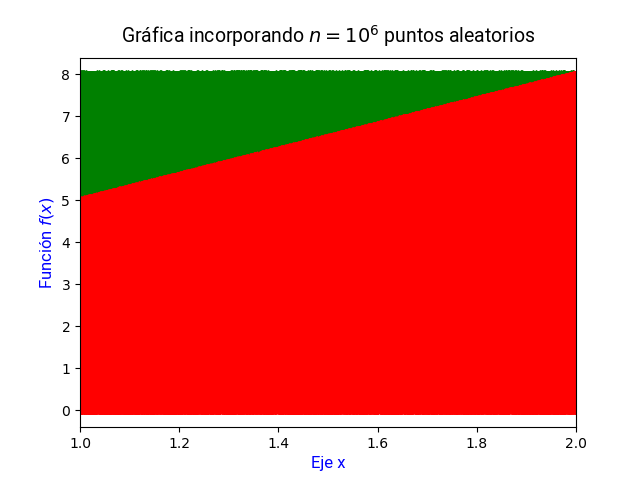
\includegraphics[scale=0.55]{Imagenes/area_puntos_06.png}
    \caption{El resultado del cálculo de la integral es exacto.}
\end{figure}
\end{frame}
% \begin{frame}
% \frametitle{Gráfica del error vs. número de muestras}
% \begin{figure}
%     \centering
%     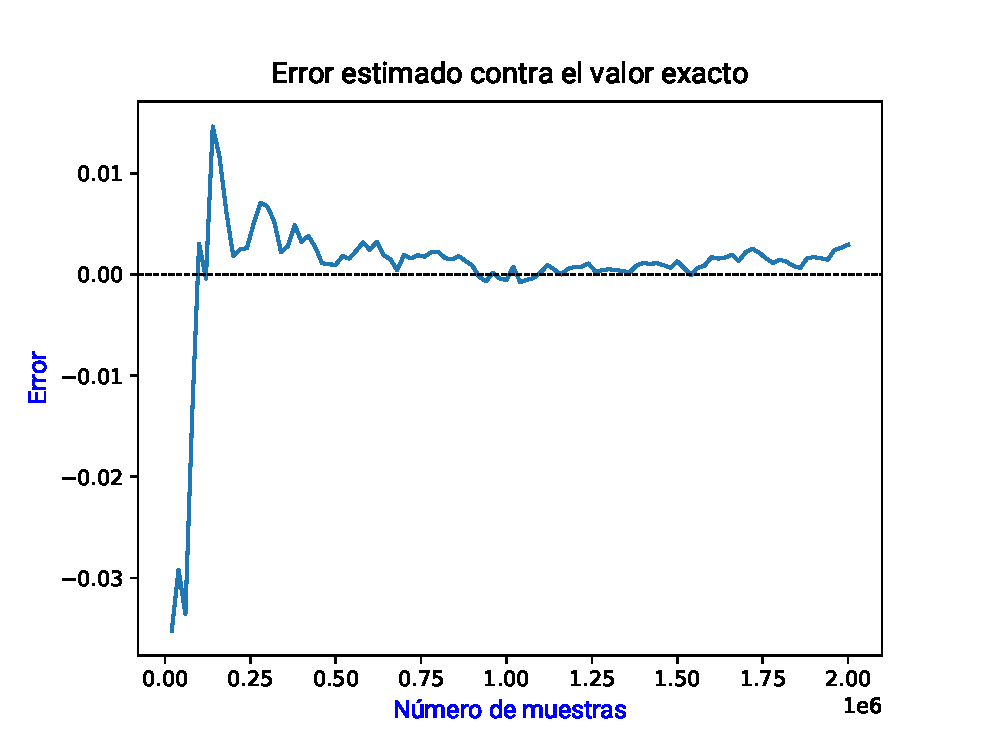
\includegraphics[scale=0.55]{Imagenes/area_puntos_07_error.eps}
%     \caption{Comportamiento del error.}
% \end{figure}
% \end{frame}
\begin{frame}
\frametitle{Ejercicios a cuenta}
Incorpora una rutina de graficación para obtener las imágenes obtenidas en las secciones:
\setbeamercolor{item projected}{bg=blue!70!black,fg=yellow}
\setbeamertemplate{enumerate items}[circle]
\begin{enumerate}[<+->]
\item Secuencia aleatoria (5 gráficas, dos de ellas se obtienen con el mismo código, en dos momentos distintos)
\item Integración Monte Carlo (8 gráficas, la imagen en la diapositiva 90, es un ejemplo, no ejercicio)
\end{enumerate}
\end{frame}
\end{document}